% This is samplepaper.tex, a sample chapter demonstrating the
% LLNCS macro package for Springer Computer Science proceedings;
% Version 2.21 of 2022/01/12
%
\documentclass[runningheads]{llncs}
%
\usepackage[T1]{fontenc}
% T1 fonts will be used to generate the final print and online PDFs,
% so please use T1 fonts in your manuscript whenever possible.
% Other font encondings may result in incorrect characters.
%
\usepackage{graphicx}
\usepackage{cite}                      % needed to automatically sort the references
\usepackage{color}
\usepackage{comment}
\usepackage{url}

%%color
\usepackage{color} %ref: http://en.wikibooks.org/wiki/LaTeX/Colors
\newcommand{\hot}[1]{{\color{red} #1}}
\newcommand{\pin}[1]{{\color{blue} #1}}

% Used for displaying a sample figure. If possible, figure files should
% be included in EPS format.
%
% If you use the hyperref package, please uncomment the following two lines
% to display URLs in blue roman font according to Springer's eBook style:
%\usepackage{color}
%\renewcommand\UrlFont{\color{blue}\rmfamily}
%
\graphicspath{{figures/}{pictures/}{images/}{./}} % where to search for the images

\begin{document}
%
\title{ArcheryVis: A Tool for Analyzing and Visualizing Archery Performance Data}
%
\titlerunning{ArcheryVis}
% If the paper title is too long for the running head, you can set
% an abbreviated paper title here
%
\author{Zhiyuan Cheng\inst{1} \and
Zeyuan Li\inst{1} \and
Zhepeng Luo\inst{2} \and \\
Mayleen Liu\inst{1} \and 
Jonathan D'Alonzo\inst{1} \and 
Chaoli Wang\inst{1}%\orcidID{0000-0002-0859-3619}
}
%
\authorrunning{Z. Cheng et al.}
% First names are abbreviated in the running head.
% If there are more than two authors, 'et al.' is used.
%
\institute{University of Notre Dame, Notre Dame, IN 46556\\
%\email{\{zcheng6,zli28,mliu5,jdalonzo,htrinh,chaoli.wang\}@nd.edu}\\ \and
\email{\{zcheng6,zli28,mliu5,jdalonzo,chaoli.wang\}@nd.edu}\\ \and
Columbia University, New York, NY 10027\\
\email{zl3092@columbia.edu}}

%
\maketitle              % typeset the header of the contribution
%
\begin{abstract}
We present ArcheryVis, a tool for analyzing and visualizing archery performance data collected from two elementary school trainees over a year. The goals are to digitally archive their training target papers, automatically detect and calibrate shots, and analyze their performance via a visual interface. We achieve automatic shot detection using a deep neural network, compute scores and relevant statistical measures, and design coordinated multiple views for interactive user exploration. Experimental results demonstrate the effectiveness of ArcheryVis.

\keywords{Archery performance \and Shot detection \and Visual interface.}
\end{abstract}
% 

\section{Introduction}

Archery is a popular sport enjoyed by people around the world. 
While it may not be as widely practiced as some mainstream sports, its popularity has grown steadily and holds a significant place in recreational and competitive circles. 
Our motivation for developing a tool that analyzes and visualizes archery performance data stemmed from a real scenario with two elementary school trainees (a boy and a girl). 
They began weekly training at a local archery shop/club in the third grade. 
Alternatively, they practiced with target papers for one week and 3D animal targets for another week. 
Later on, they also received additional training sessions over weekends. 
Over one year, they each completed 36 target papers, totaling 72 papers (63 25"$\times$25" and 9 17"$\times$17"). 
These papers are bulky, making them inconvenient to store long-term. 
More importantly, it is challenging for the trainees and their trainer to analyze their performance over time, let alone make a comparison between them. 
As they continued their training, more target papers collected only exacerbated the challenges of post hoc analysis. 

In response, we present ArcheryVis, which outlines the following steps to streamline the process of archiving, analyzing, and visualizing archery performance data. 
First, instead of carrying target papers around, it is much more convenient to take photos of target papers on-site via smartphones for digital recording. 
With raw data stored as digital images, we want to develop a solution that automatically ``scans'' each image to detect landmarks (i.e., the rings, center, and shots) from which we can reliably calibrate shots, compute scores, and gather relevant statistical measures. 
After that, we have the necessary information to ``reconstruct'' the target papers on the screen for performance analysis. 
We design and develop a set of coordinated multiple views to support effective visual exploration and comparison of the archery performance data. 

\section{Related Work}
\label{sec:rw}

\subsection{Archery Performance Analysis}
 
High-performance shooting in archery is the ability to accurately shoot an arrow at a given target. 
% 
Researchers have long explored various physiological, psychological, biomechanical, and kinematic factors contributing to archery performance. 
%
Vendrame et al.\ \cite{Vendrame-SB22} conducted a systematic review (41 studies spanning 35 years) of archery performance assessment. The investigation of the influence of a wide range of physiological and kinematic parameters revealed that high-performance archers maximize postural stability and develop personal strategies for muscular activation and time management.

An early work by Landers et al.\ \cite{Landers-RQES86} examined the physical, psychological, and perceptual/visual variables using an overall hierarchical regression model and identified seven important variables related to elite archers' shooting performance. 
%Using an overall hierarchical regression model, they identified seven variables (relative leg strength, reaction time, depth perception, endomorphy, imagery usage, confidence, and focus on past mistakes) associated with archery performance. 
%
Soylu et al.\ \cite{Soylu-HMS06} recorded surface electromyography (EMG) signals of musculus flexor digitorum superficialis and extensor digitorum of archers during archery shooting to compare the repeatability of EMG linear envelopes of archery groups. 
%
Tinazci~\cite{Tinazci-PE11} investigated the relationships between physiological and mechanical dynamics during arrow releasing in archery with the quality of the arrow shot, involving four elite male archers.
%
Kim et al.\ \cite{Kim-TJSCR15} explored the mental, skill, and fitness factors affecting archery performance. They met with experts and conducted a confirmatory factor analysis and the analytic hierarchy process to identify the most important factors. 
%
Quan and Lee~\cite{Quan-KJSB16} studied the relationship between aiming patterns and scores. The aiming pattern was defined using averaged acceleration data measured from accelerometers attached to the body. They employed regression analysis with dynamic time warping to explore the effective way to raise scores in archery shooting. 
%
Kim et al.\ \cite{Kim-IJERPH21} performed a meta-analysis study to investigate the effectiveness of psychological skills training interventions for archers in Korea. Their study revealed that psychological skills training for archers is effective, and the player level and training period are crucial factors. 

Recent works also explore machine learning and visualization techniques for archery performance analysis.
%
Muazu Musa et al.\ \cite{Muazu-Musa-SS19} leveraged artificial neural network and k-nearest neighbor classification techniques to forecast and scout high-performance archers. The machine learning techniques were trained on physical fitness and motor skill parameters, including hand grip, vertical jump, standing broad jump, static balance, upper muscle strength, and core muscle strength.
%
Kawaguchi et al.\ \cite{Kawaguchi-AH20} proposed a system to easily search differences in multiple trial motions of the same archer. The time-series data was collected using the angular velocity sensor attached to the bow. Dynamic time warping was utilized to determine the similarity of multiple shots. 

Unlike all the above works, we only collected archery data directly related to target performance, excluding any contributing factors. 
This is similar to Kolayis et al.\ \cite{Kolayis-PSBS14}, which manually assesses target performance in archery, focusing on the error distributions using the one-sided ANOVA and chi-squared tests. 
% 
The differences are that our ArcheryVis detects shots automatically and emphasizes the analytical capability via visualization, which is not presented in prior research to our best knowledge. 

\subsection{Archery Scoring Apps}

Even though visualization research on archery performance data is scarce, several archery scoring apps are available for training or competition, including MyTargets Archery, Archery Companion, iArchery, and Archer's ToolBox. 
%
MyTargets Archery allows users to store and manage their equipment, noting their bows, arrows, sight marks, and relevant information. 
A sight mark is a reference point that archers use to adjust the position of their sight's pins or reticles when aiming at different distances. 
%A sight mark in archery refers to a specific setting on a bow's sight that corresponds to a known distance. Archers adjust their sight's pins or reticles based on these marks, allowing them to aim accurately at targets placed at different distances without needing to estimate the range. It's a crucial technique that enhances shooting consistency and accuracy in various archery disciplines. 
Scoresheets are available for different rounds with color coding to the target. 
%
Archery Companion lets users track scores and sight marks and choose the round they shoot. The scoresheet only shows the arrow values and end score.
%
With iArchery, users can log their round scores, sight marks for specific equipment, and personal bests. They can select the round, bow type, and date shot in the scoresheet.
%
Finally, Archer's ToolBox provides similar functions as other apps. Besides, this app allows users to send scores to their club for verification.

All these apps are designed for manual scoring and training journals. 
Our ArcheryVis aims to detect shots and calculate scores from raw image input automatically. 
It goes beyond scoresheets by reconstructing the results for ``in-place'' visual analysis. 
Moreover, it supports visual comparison across trainees, a missing feature in these apps. 
 
\section{Data Collection, Processing, and Analysis}

\subsection{Data Collection}

We asked the two elementary school trainees to take a photo of their respective completed target paper using a smartphone after each training session. The photo was taken so that the camera's view was approximately perpendicular to the target paper, and the target's center (i.e., the bullseye) was nearly at the center of the camera's image plane. Each photo was taken under a similar indoor lighting condition and was cropped using the smartphone's built-in camera app. The collected digital images were uploaded to a shared Google folder each time for subsequent processing and analysis.

\begin{figure*}[htb]
\begin{center}
$\begin{array}{c@{\hspace{0.25in}}c}
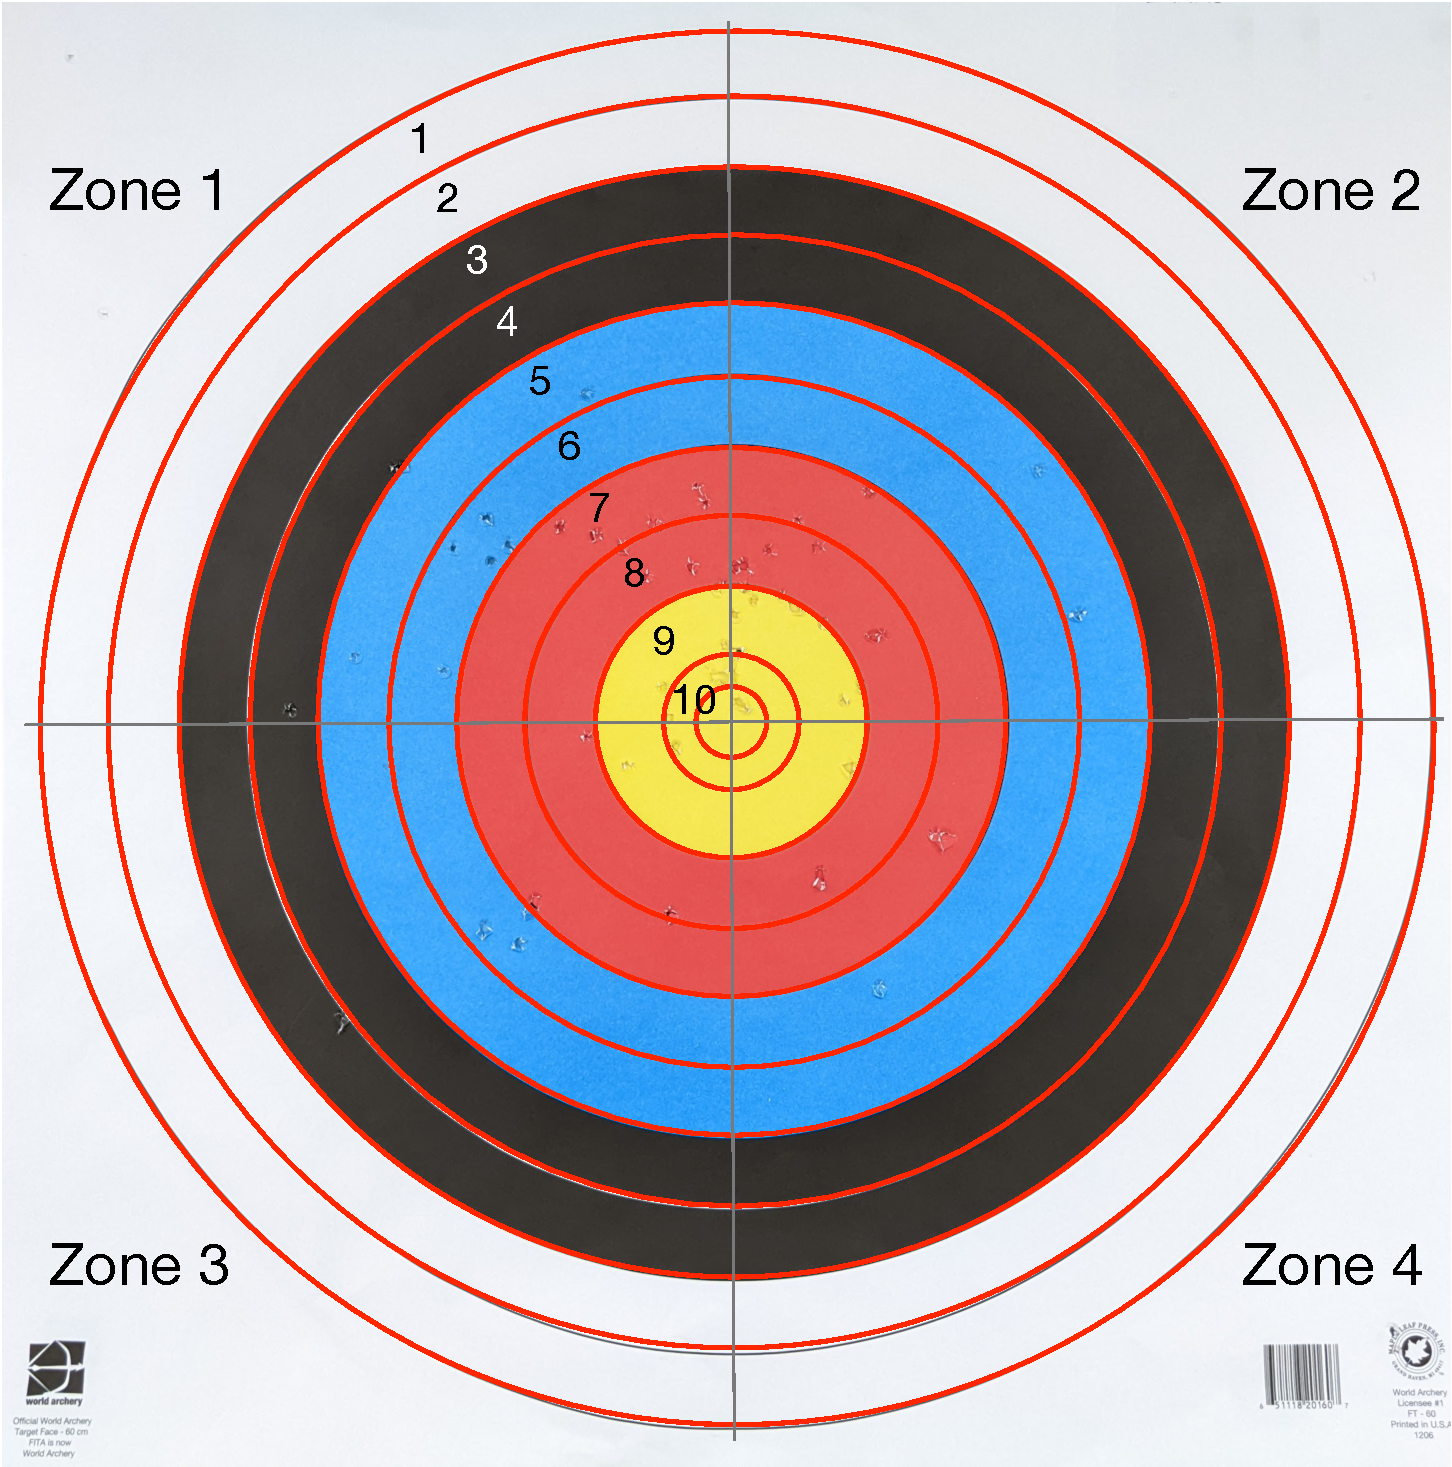
\includegraphics[height=1.75in]{figures/ring-detection.pdf}&
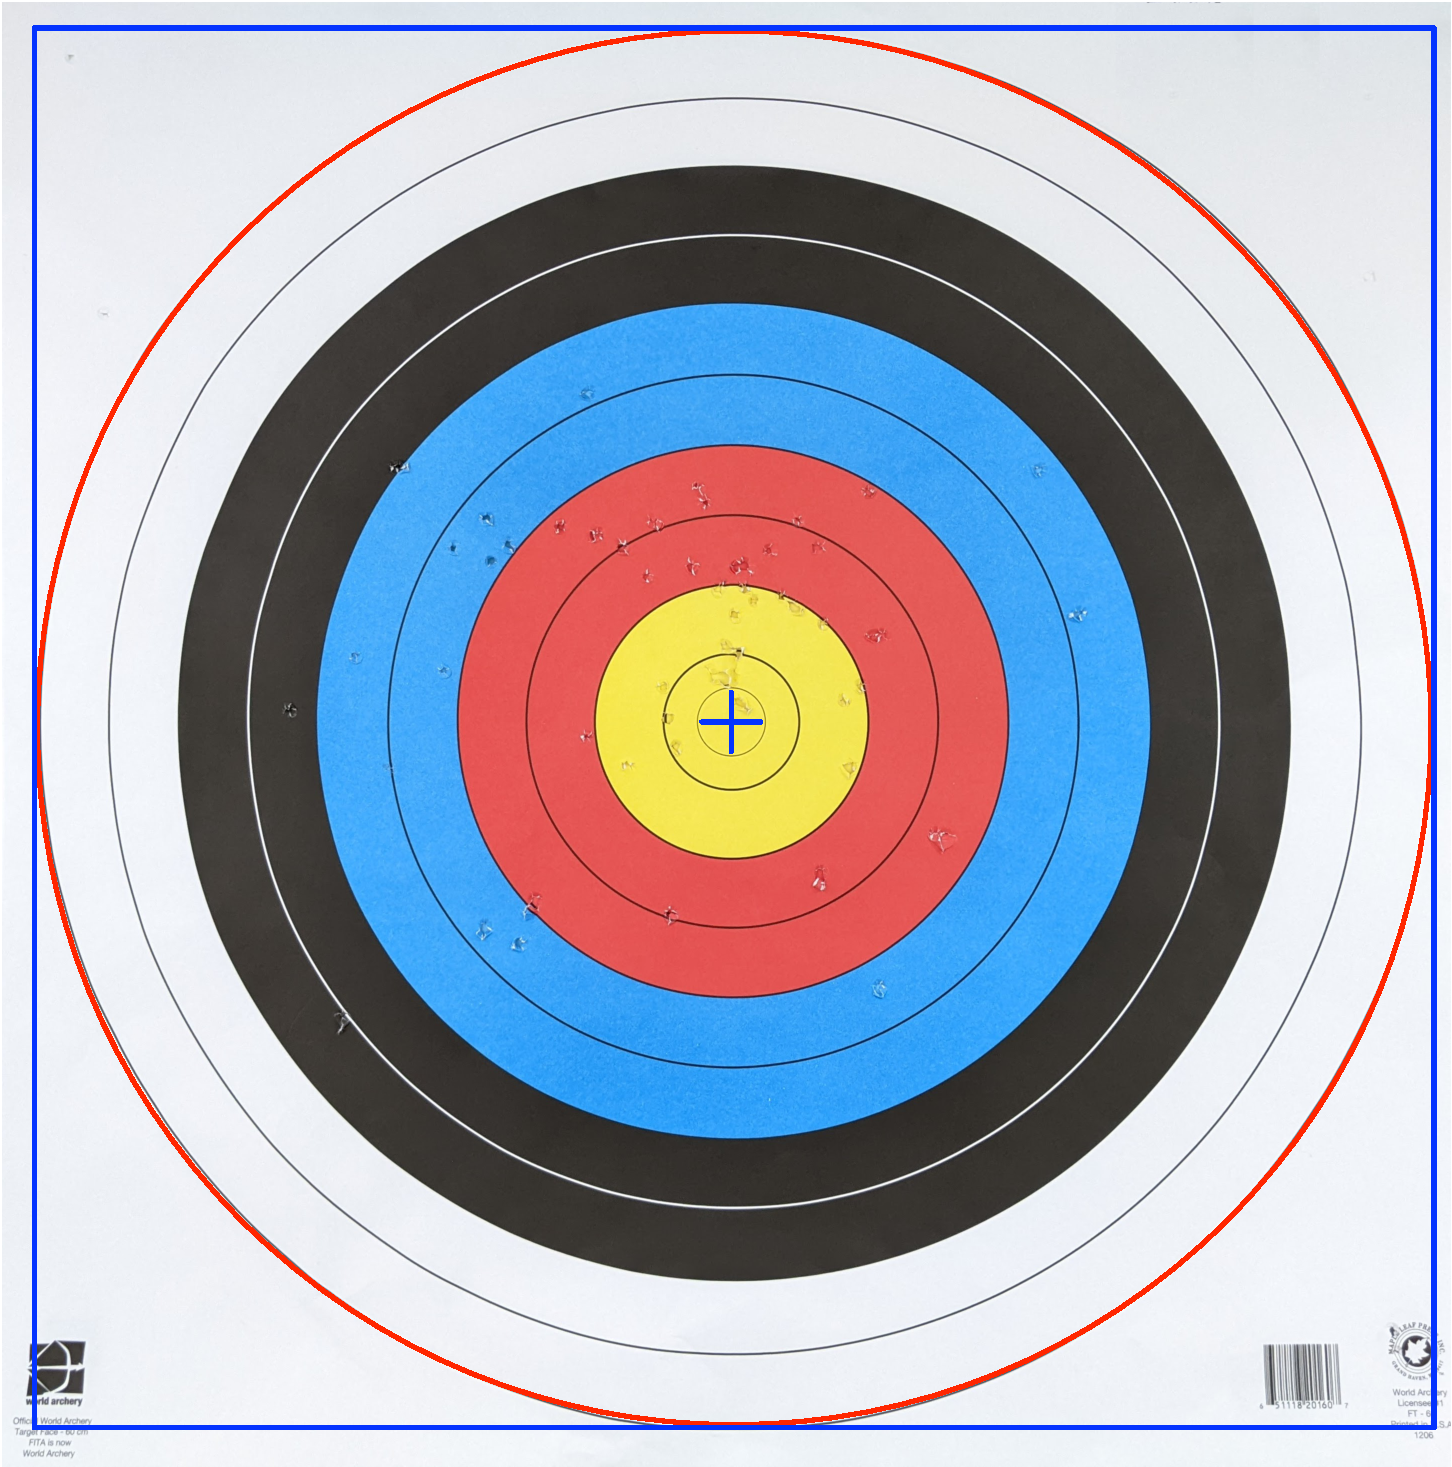
\includegraphics[height=1.75in]{figures/center-detection.pdf}\\
\mbox{(a)} & \mbox{(b)}
\end{array}$
\end{center}
\caption{(a) and (b) show detected rings and the center of an archery target paper.}
\label{fig:ring-center}
\end{figure*}

\subsection{Ring and Center Detection}

We apply the popular Hough transform~\cite{Duda-CACM72} to detect the rings due to its robustness in detecting geometric shapes even in the presence of noise. It transforms points in the image space to a parameter space, where the geometric shape's parameters (such as slope and intercept for lines or center and radius for circles) can be more easily detected. 
%The transformation involves mapping each point in the image space to a curve or peak in the parameter space. 
%For example, in the case of line detection using the Hough transform, each edge pixel in the image space is transformed into a sinusoidal curve in the parameter space. The intersection of these curves corresponds to the parameters of the lines present in the image.
%
%By thresholding and analyzing the parameter space, one can identify the most significant curves or peaks, representing the geometric shapes of interest. These peaks can then be back-transformed to the image space to obtain the detected lines or circles.
%
Figure~\ref{fig:ring-center} (a) shows an example of the ring detection result. We can see that the detected rings (shown in red) overlap well with the ring boundary pixels on the image. Some ring pixels have slight offsets (e.g., the bottom part of Figure~\ref{fig:ring-center} (a)) as they are distorted. This is due to two reasons. First, the target paper was not placed perfectly flat when the photo was taken. Second, the camera's view was not exactly perpendicular to the target paper. 

We do not rely on the Hough transform for center detection because it is a small cross on the target paper (refer to Figure~\ref{fig:ring-center} (a)). Instead, we get the bounding box of the outmost ring and treat its center as the center of the target. Figure~\ref{fig:ring-center} (b) shows the bounding box and its center (shown in blue). 

\begin{figure*}[htb]
\begin{center}
$\begin{array}{c@{\hspace{0.1in}}c@{\hspace{0.1in}}c}
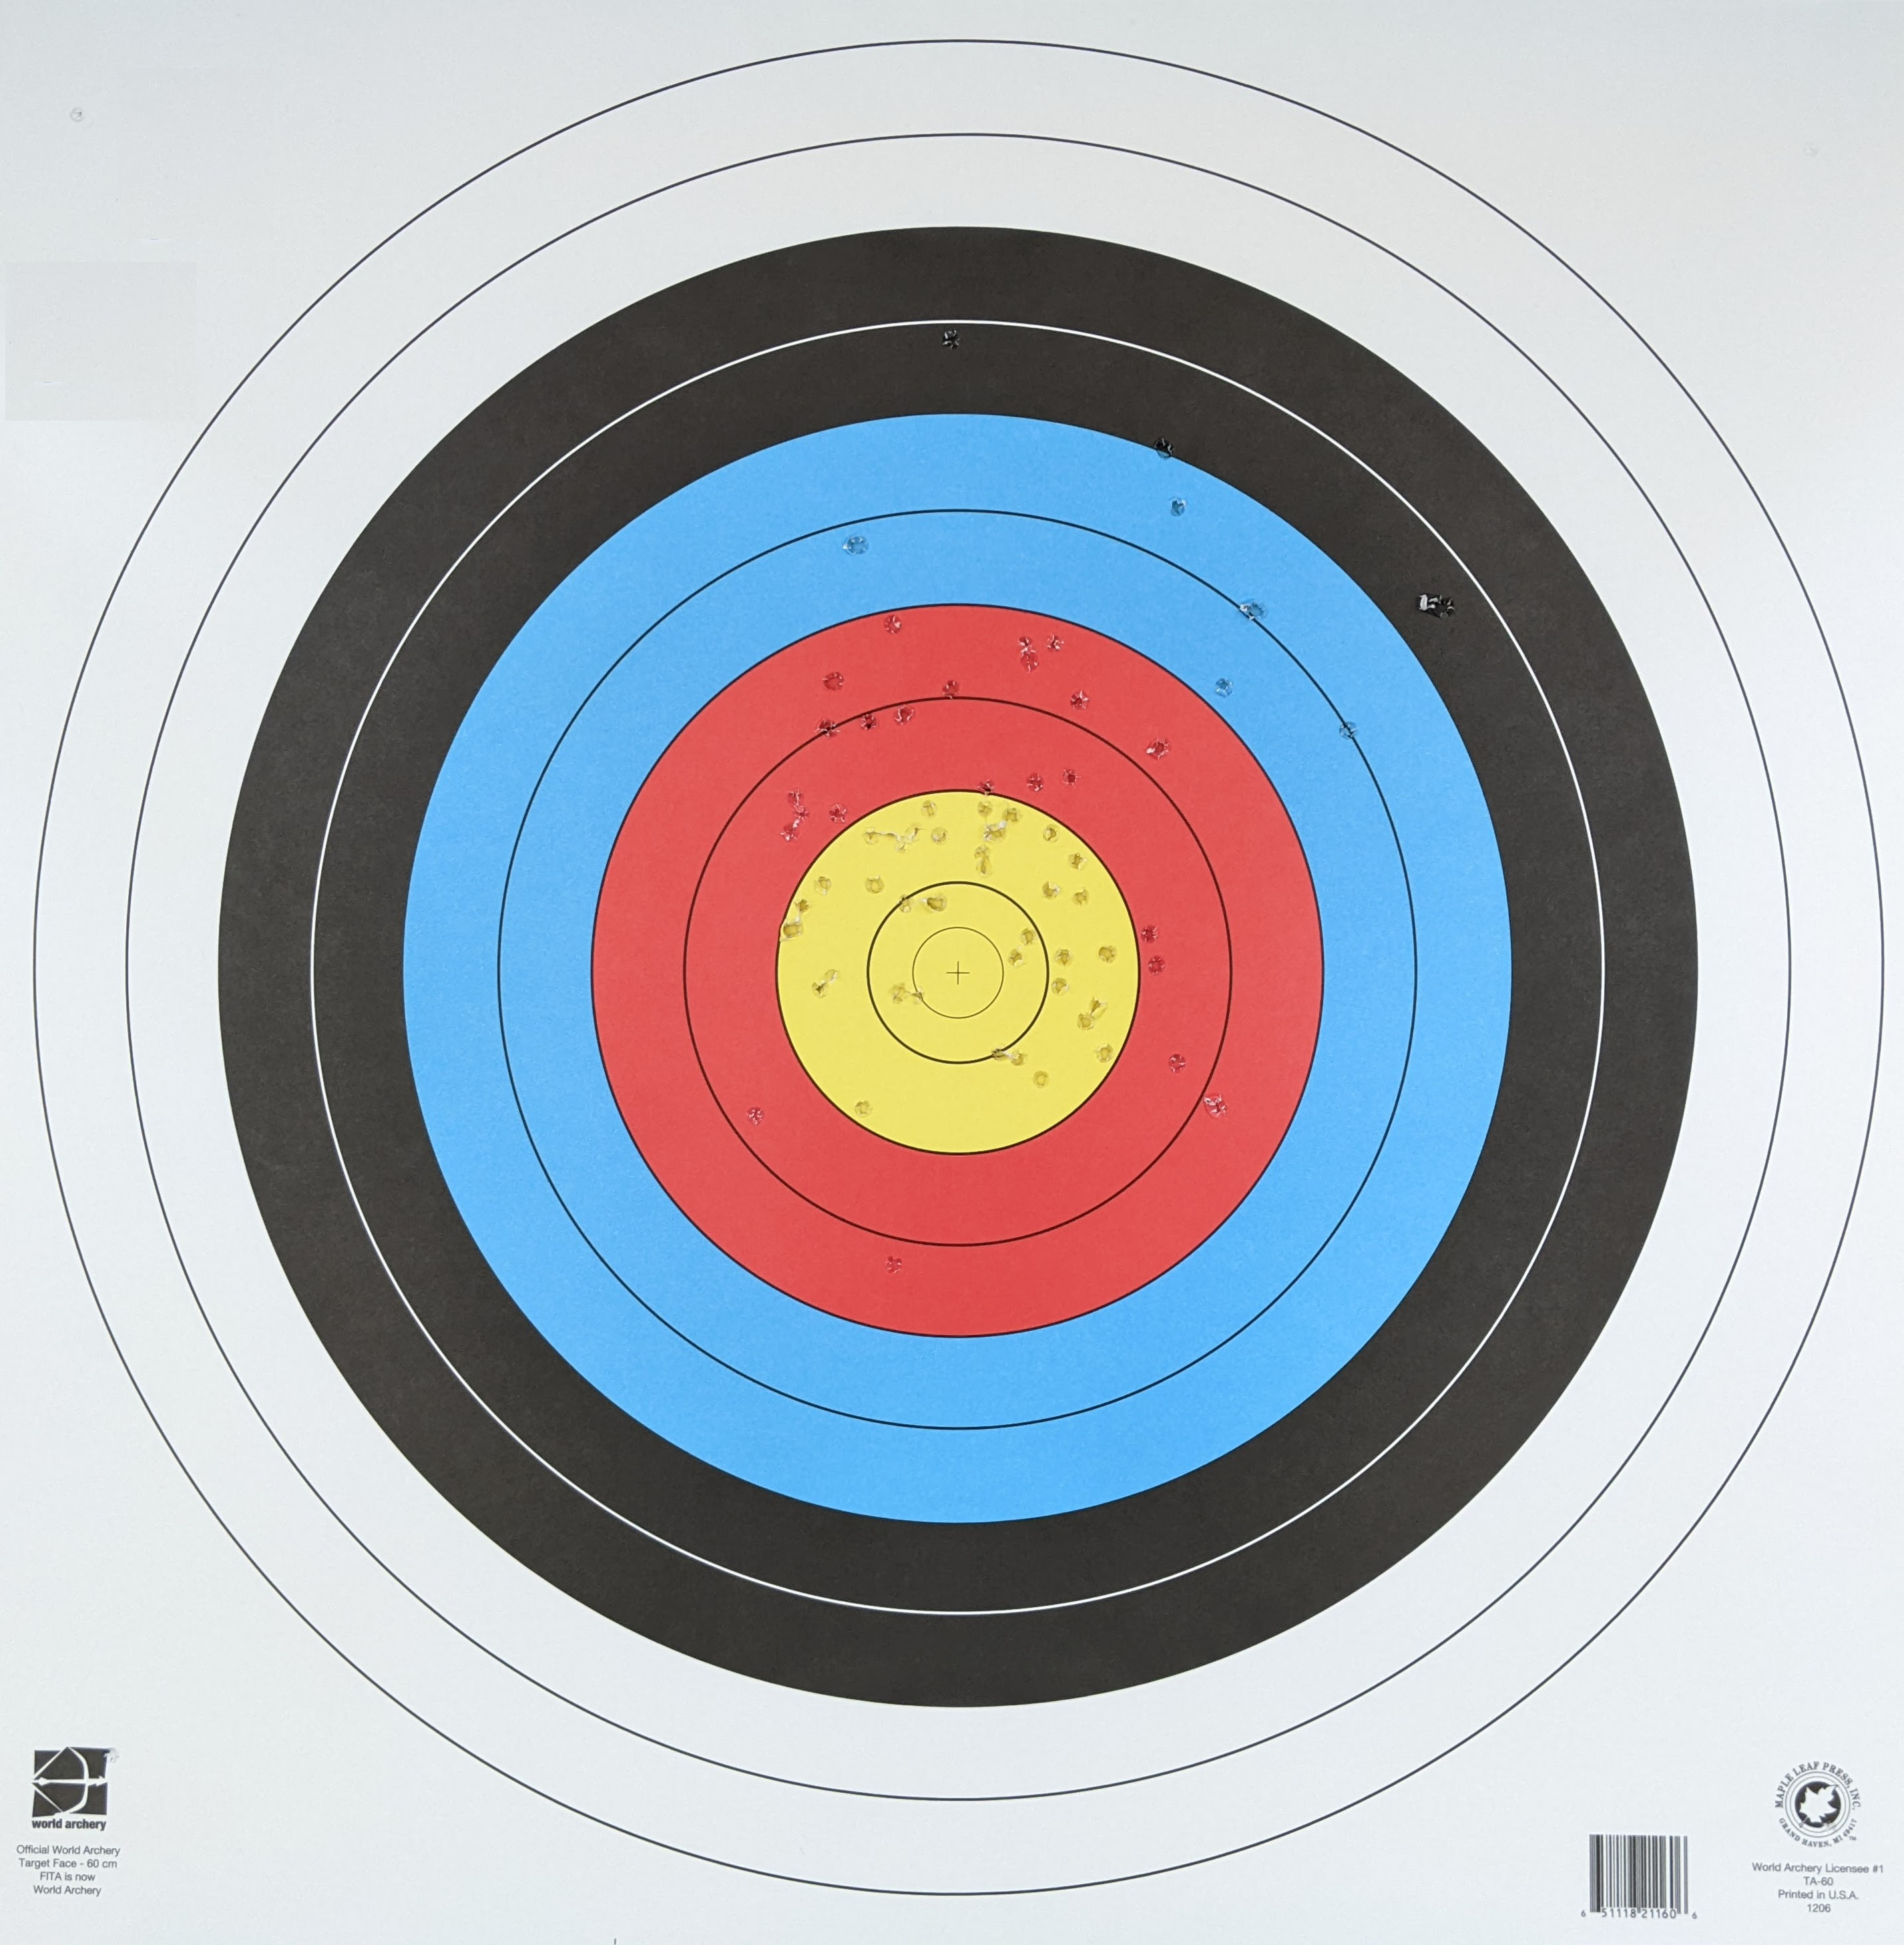
\includegraphics[height=1.35in]{figures/leo-2022-05-11.jpg}&
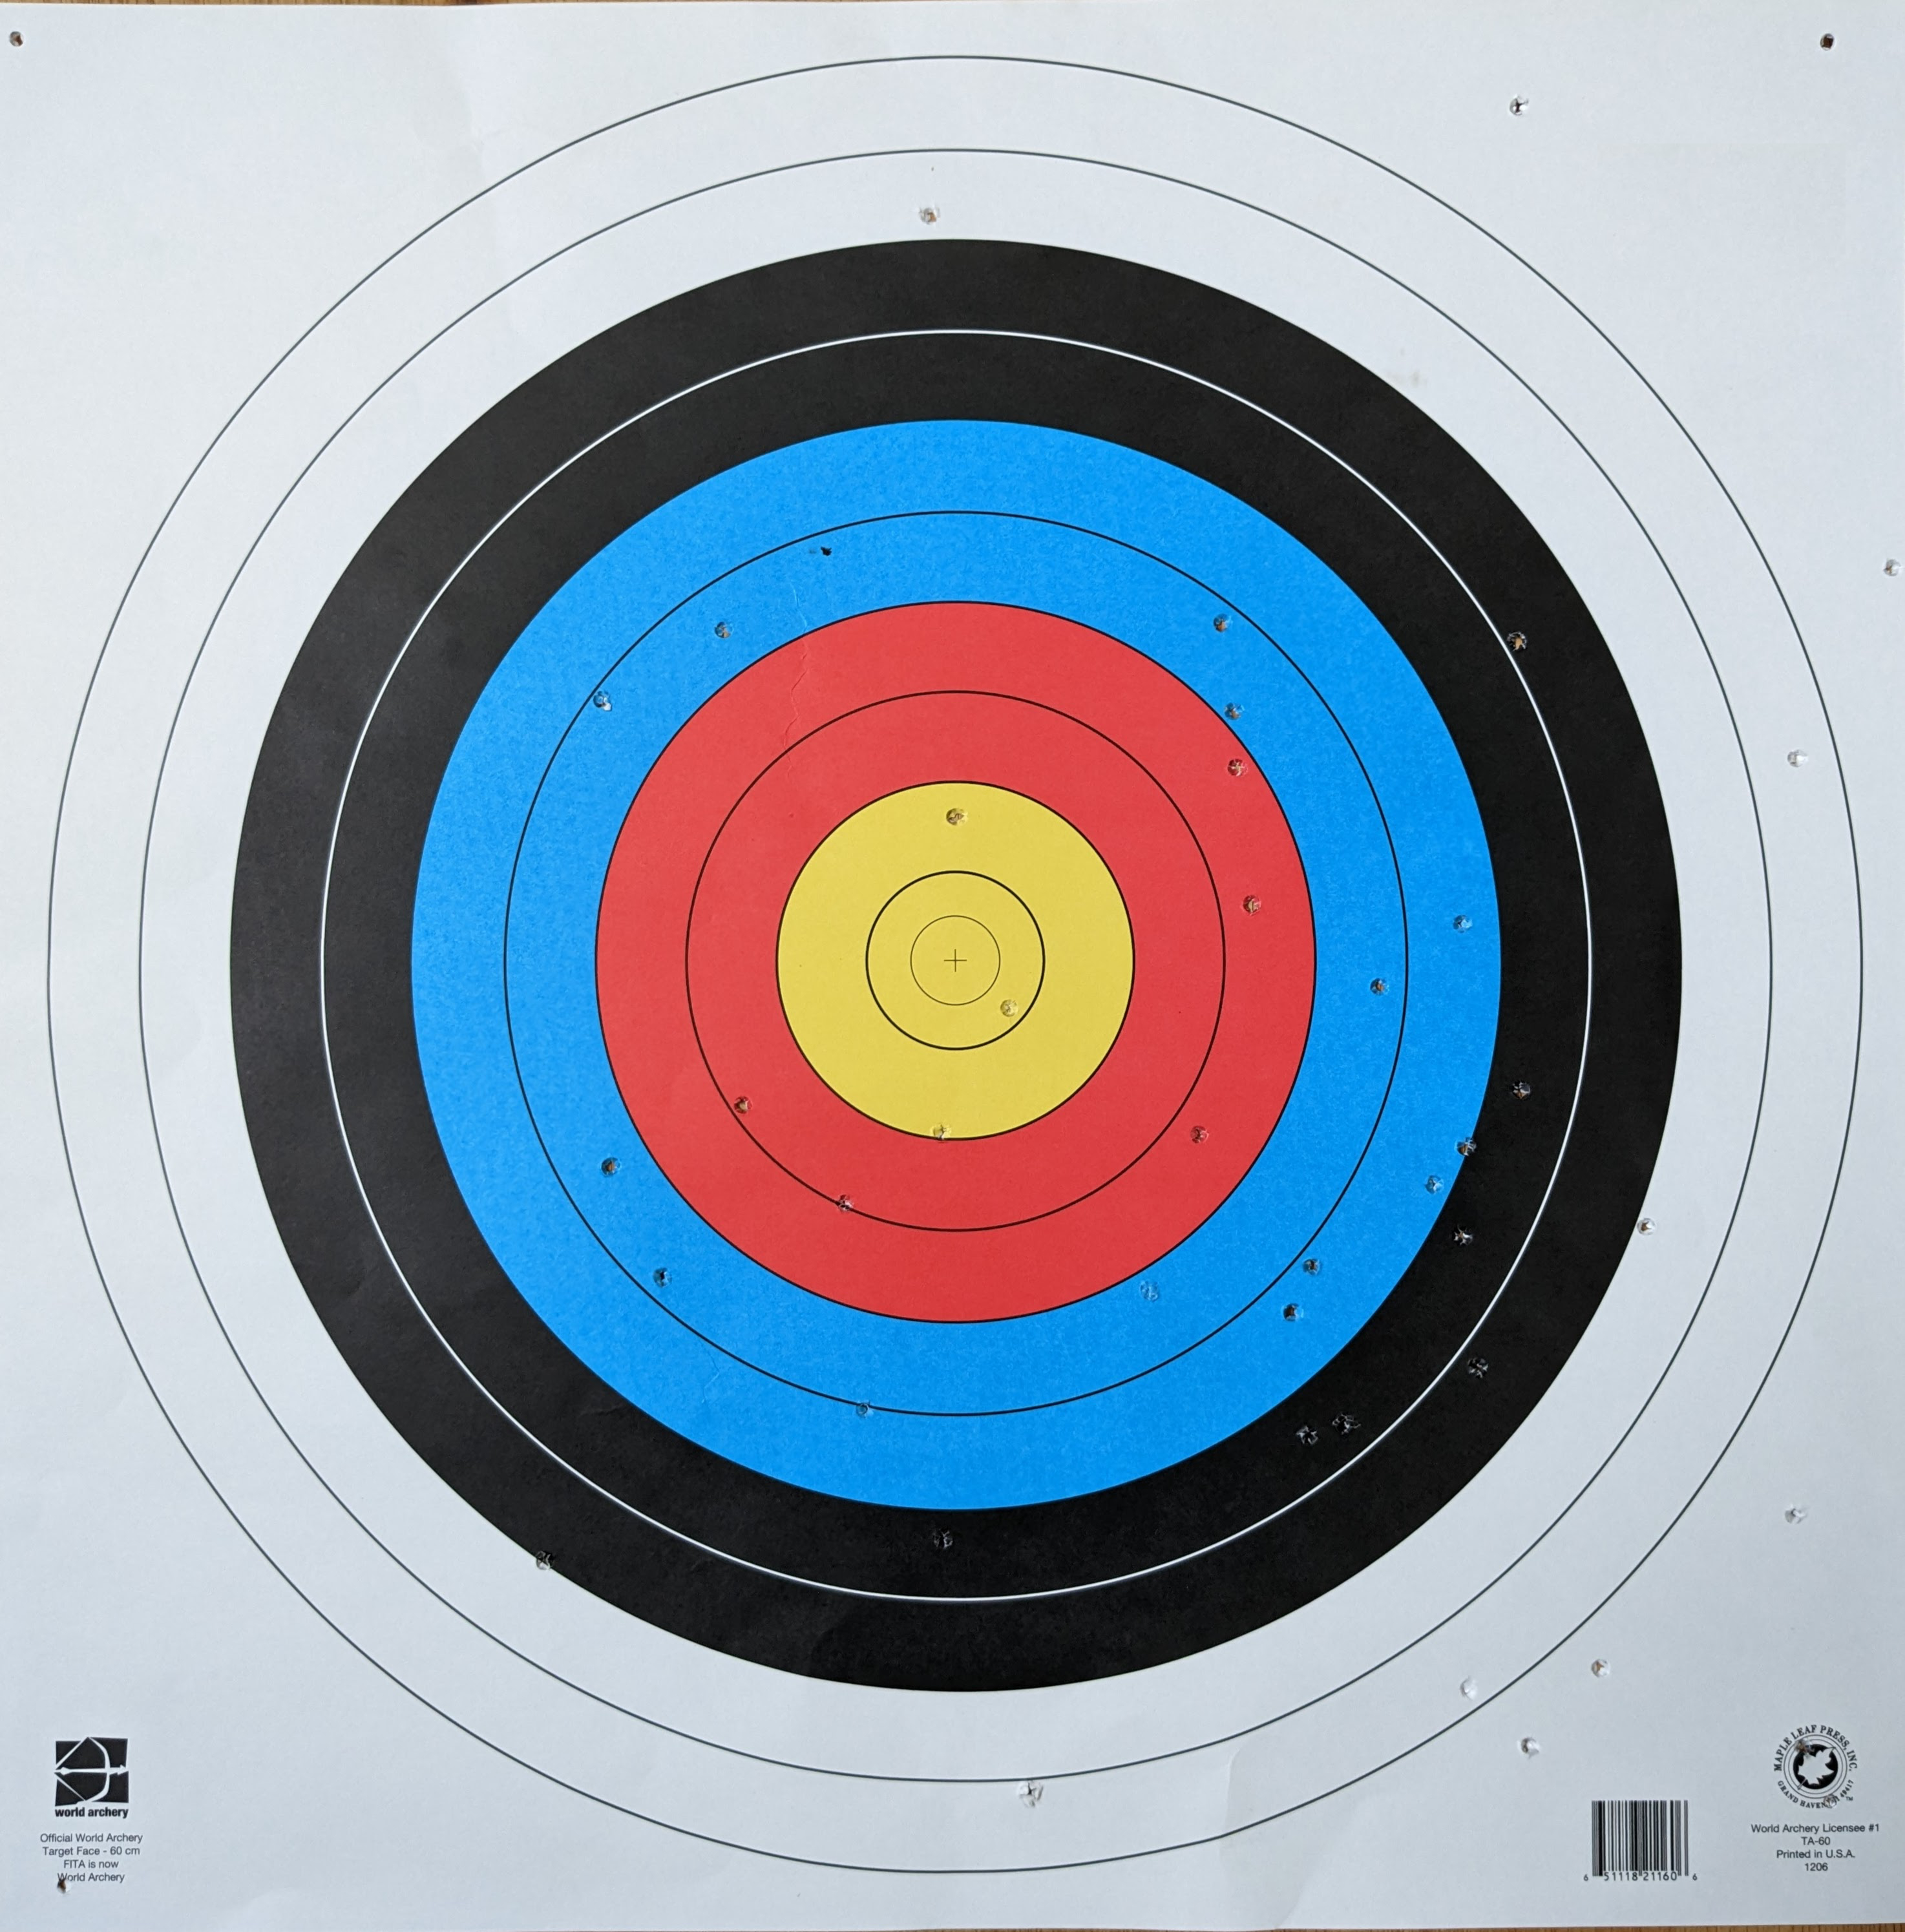
\includegraphics[height=1.35in]{figures/leo-2022-12-13.jpg}&
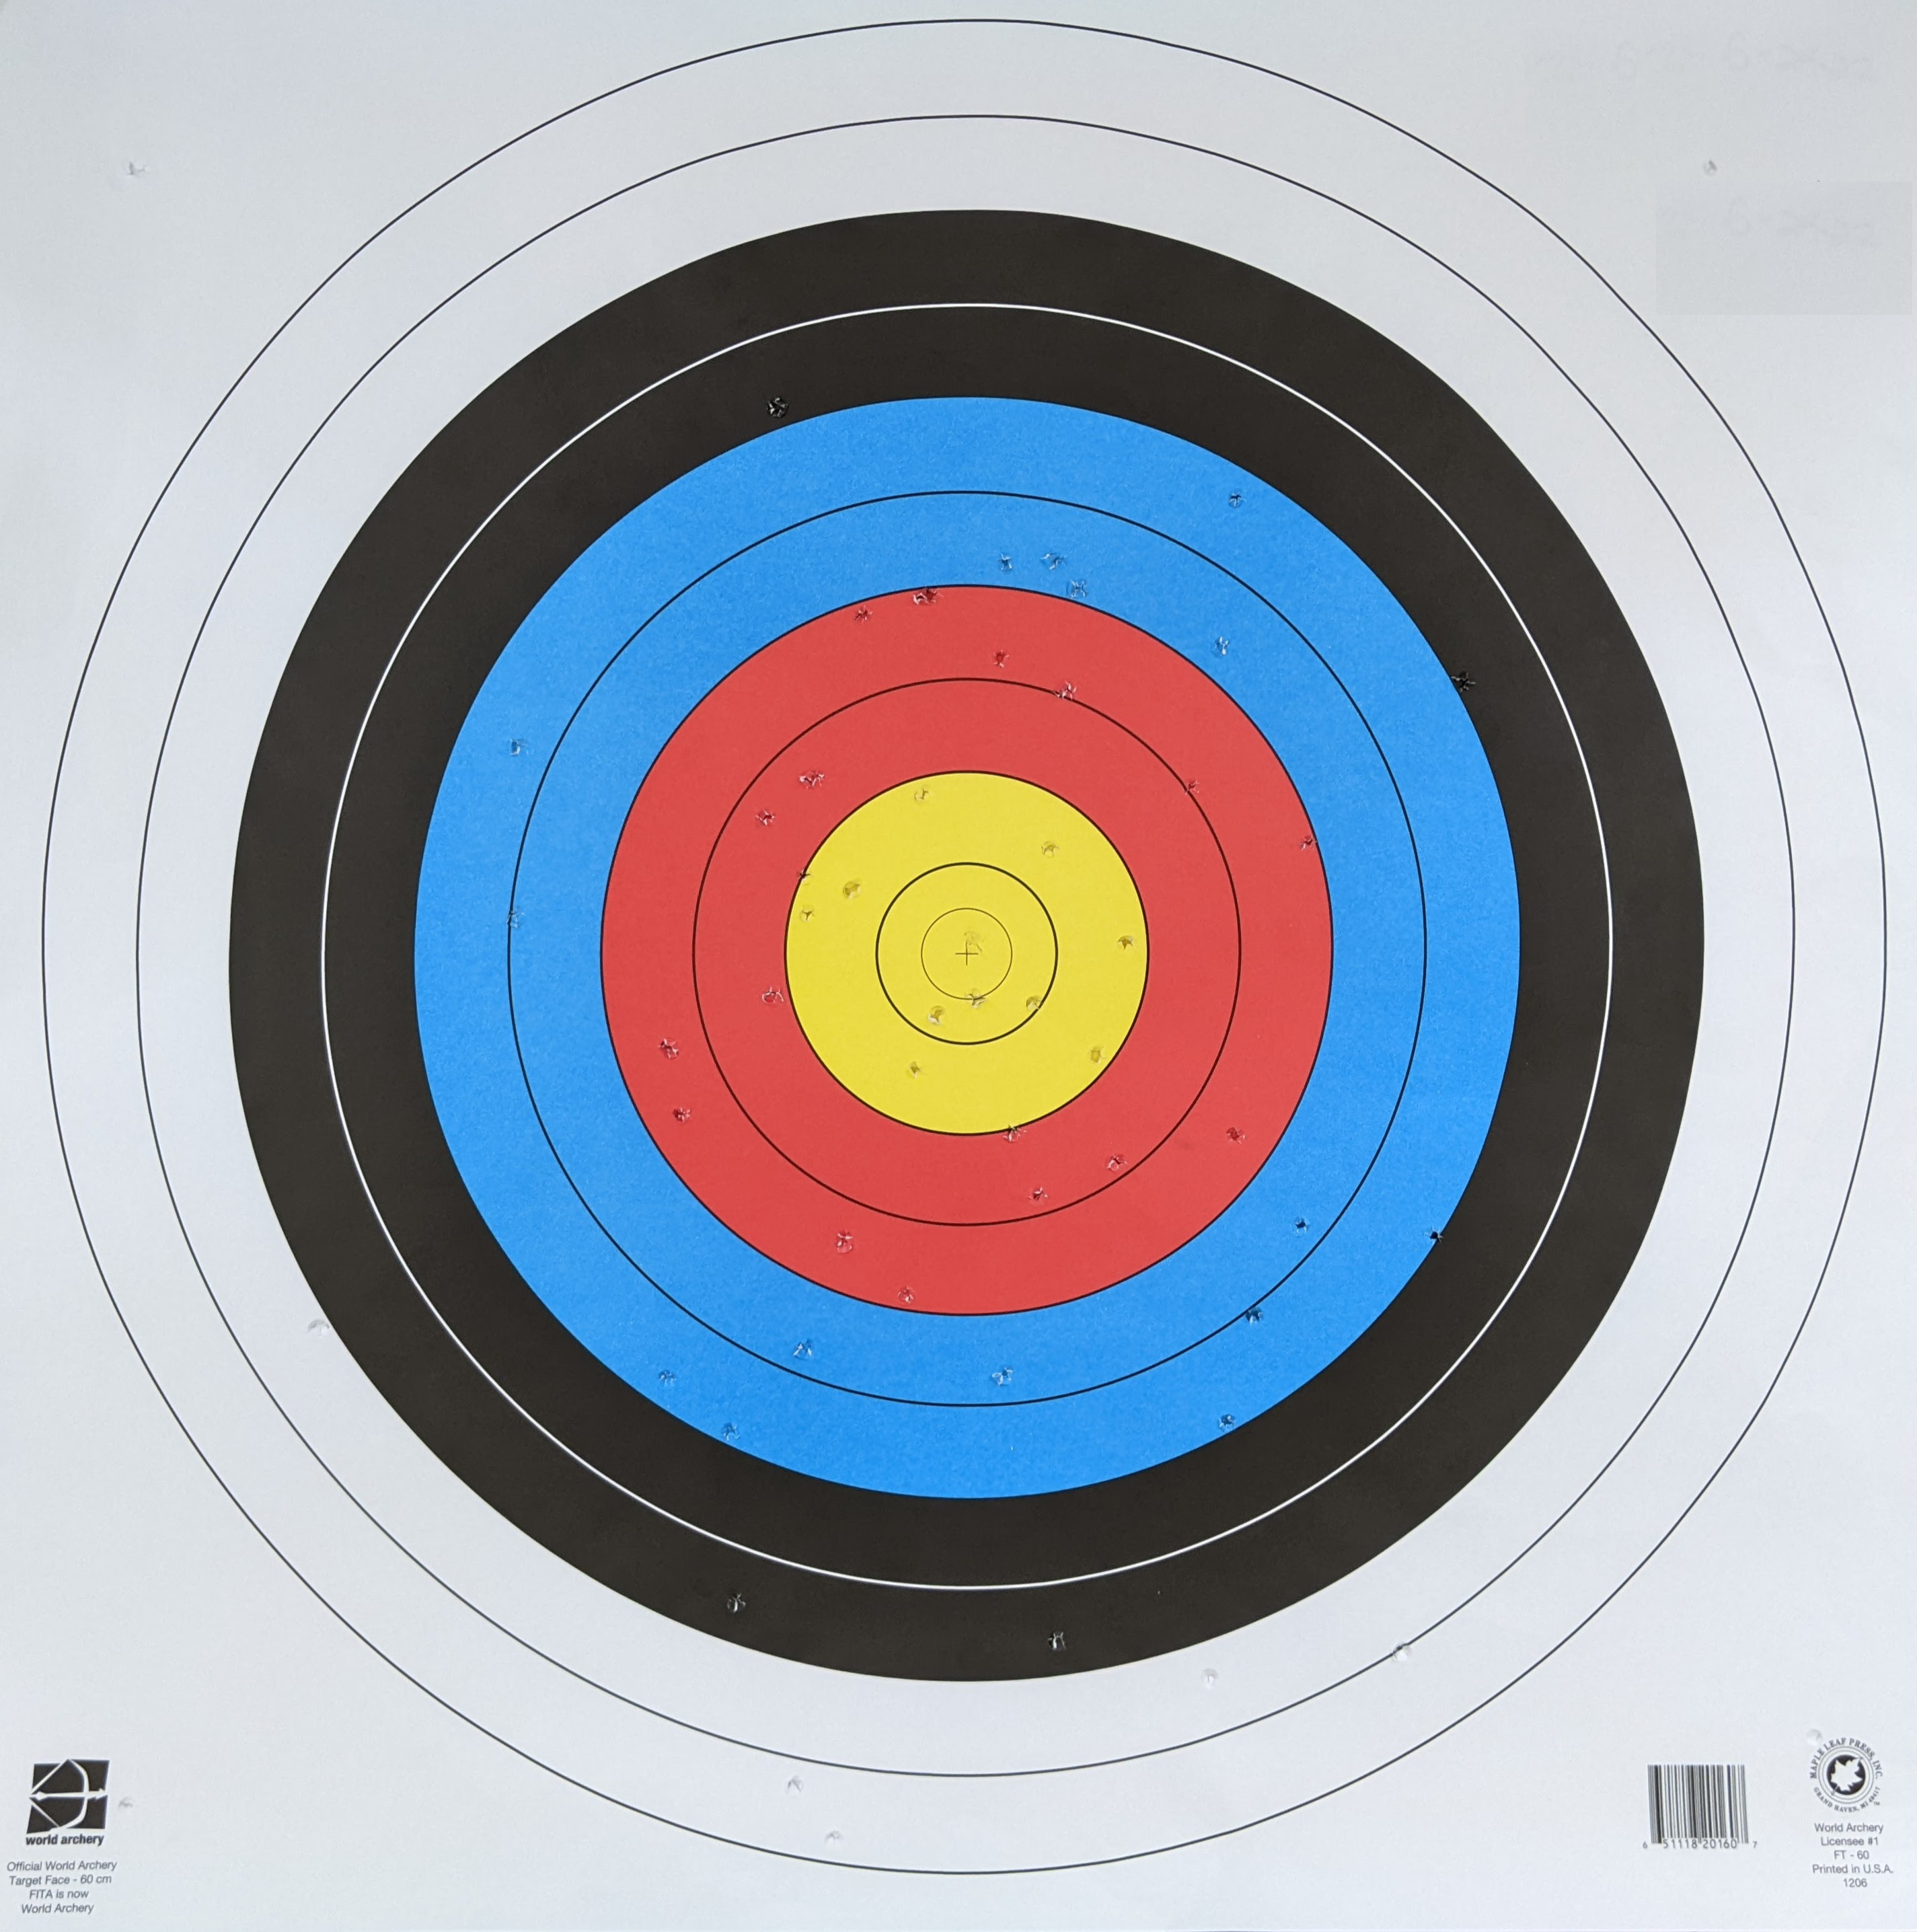
\includegraphics[height=1.35in]{figures/leo-2022-05-26.jpg}\\
\mbox{(a)} & \mbox{(b)} & \mbox{(c)}\\
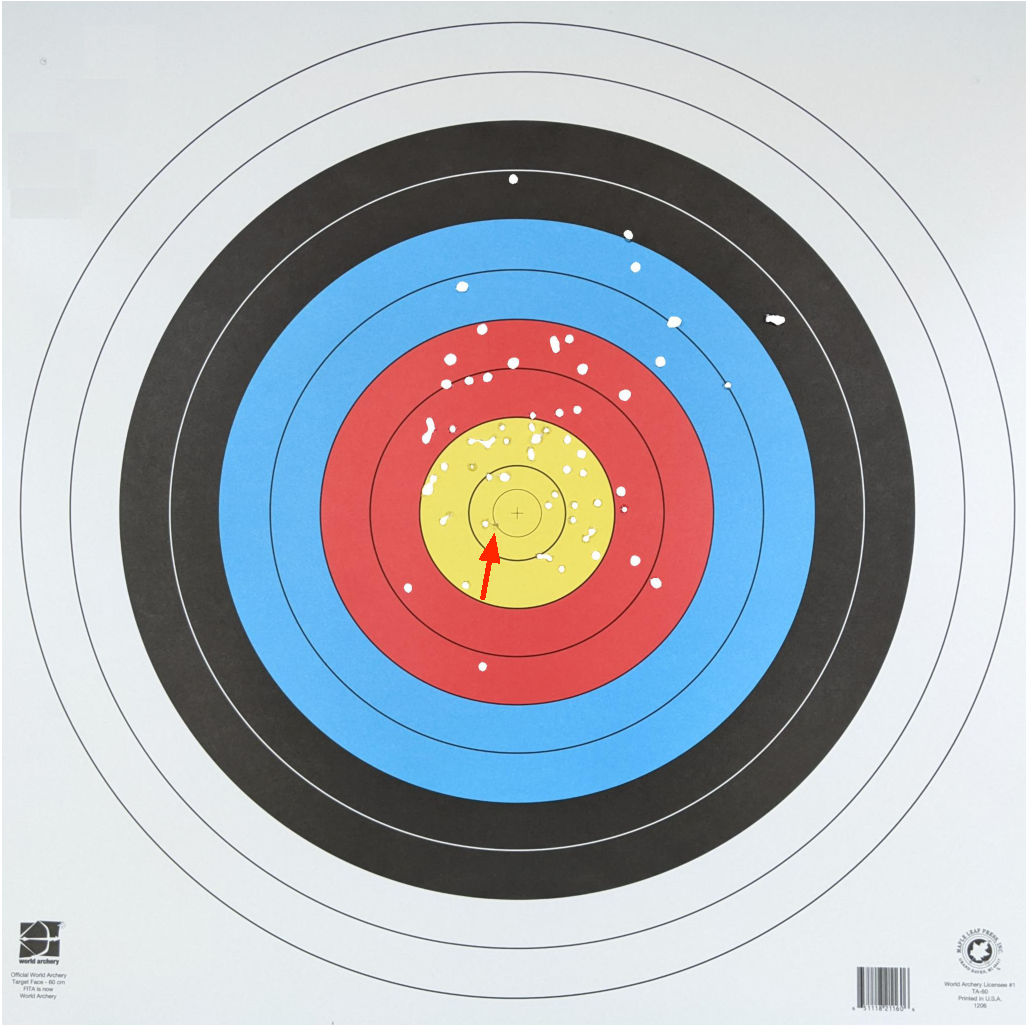
\includegraphics[height=1.35in]{figures/shot-detection-train.pdf}&
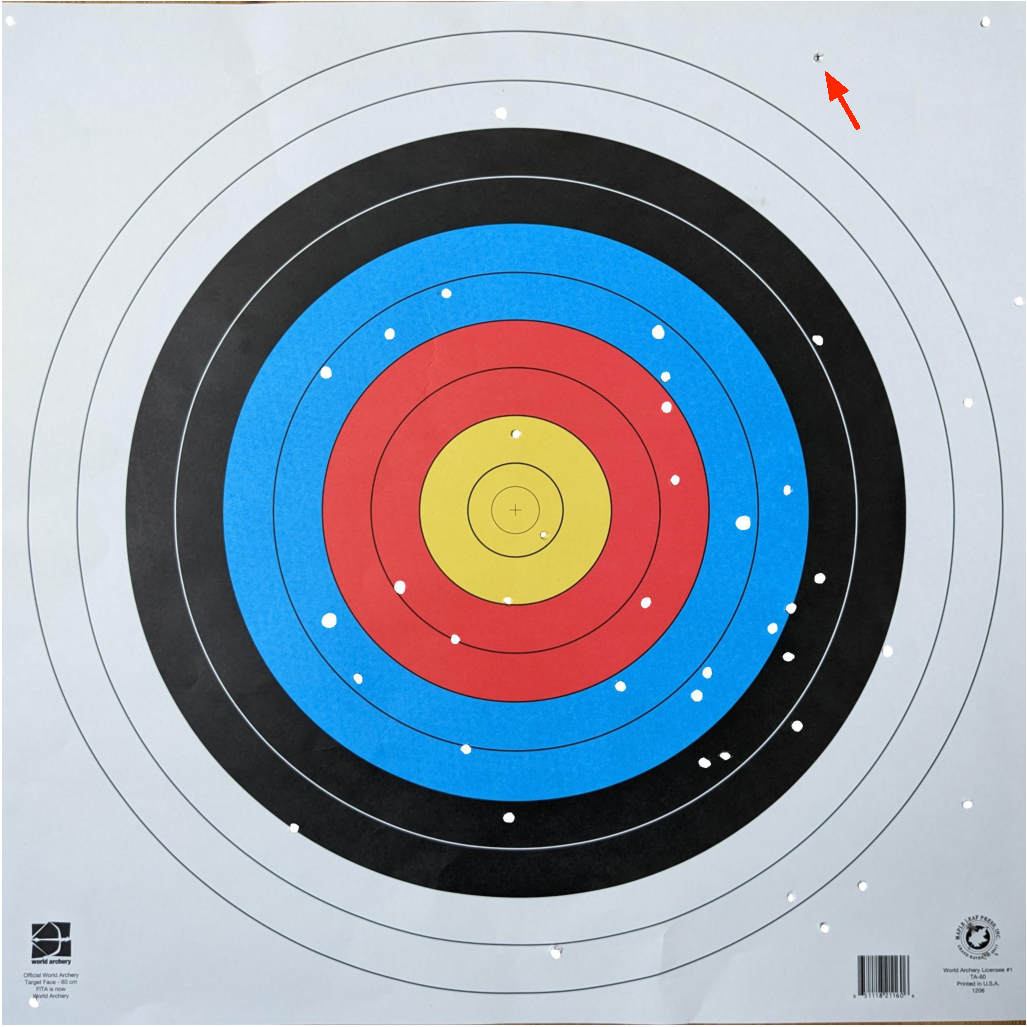
\includegraphics[height=1.35in]{figures/shot-detection-test.pdf}&
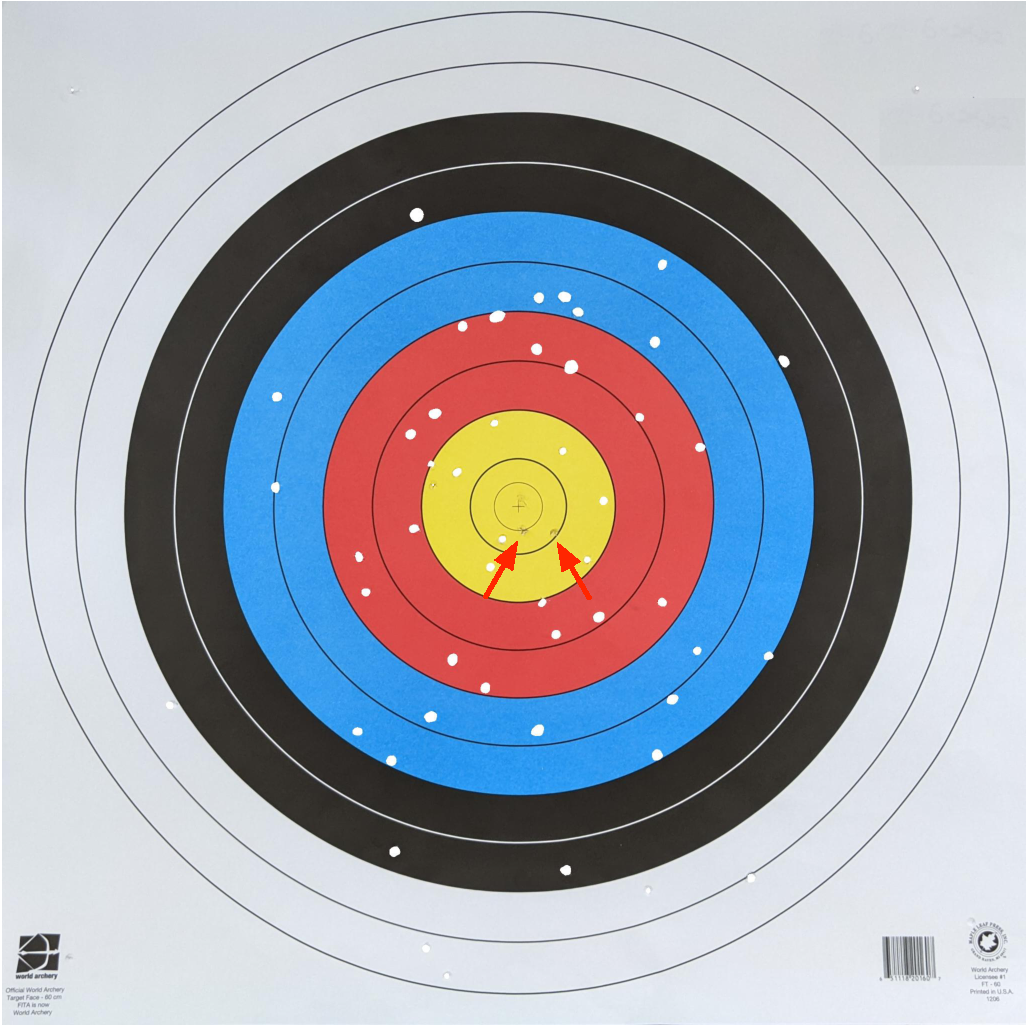
\includegraphics[height=1.35in]{figures/shot-detection-inference.pdf}\\
\mbox{(d)} & \mbox{(e)} & \mbox{(f)}
\end{array}$
\end{center}
\caption{(a) to (c) show target papers for training, testing, and inference. (d) to (f) show respective shot detection results. False negatives are highlighted in arrows.}
\label{fig:shot-detection}
\end{figure*}
%56, 40, 52; 1, 1, 2; 98.2%, 97.5%, 96.1%

\subsection{Shot Detection and Calibration}

We treat shot detection as an image segmentation problem and apply a 2D fully convolutional network (FCN)~\cite{Long-CVPR15} to obtain segmented results where pixel blobs corresponding to foreground shots are separated from the background image. 
FCNs allow for efficient and accurate pixel-level predictions, making them valuable in applications requiring precise spatial understanding or object segmentation.
Previously, Hu et al.\ \cite{Hu-VI20} leveraged an FCN to automatically detect and segment ants from surveillance videos to explore their movement patterns.  

Unlike convolutional neural networks (CNNs) that are mainly used for classification, FCNs are designed to produce dense pixel-wise predictions by preserving spatial information.
An FCN typically follows an encoder-decoder architecture. 
The encoder extracts hierarchical features from the input image through convolutional layers. The decoder performs upsampling operations to recover the spatial dimensions lost during encoding. 
The final output of an FCN is a dense prediction map with the same spatial dimensions as the input image. Each pixel in the output map represents a class label or a probability distribution over classes, depending on the specific segmentation task.

In our scenario, the original FCN~\cite{Long-CVPR15} suffers from a loss of resolution due to downsampling. We tackle this problem by adding additional upsampling blocks to the end of each layer so that different feature levels are extracted and integrated towards the final prediction. 
%In chronological order, 
We use the first 20 images of the 72-image collection for network training. 
Each image is resized to 2048$\times$2048 pixels and manually labeled to obtain ground-truth results. 
We perform data augmentation via random cropping and rotation, producing 6000 small block samples (256$\times$256 pixels each). 
These blocks are divided into training, validation, and testing sets with 70\%, 20\%, and 10\% split. 
The network is trained using the Adam optimizer with a learning rate of $10^{-3}$. 
We set 20 epochs for training with early stopping.

Figure~\ref{fig:shot-detection} shows our shot detection results. Sampled training, testing, and inference results are displayed in (d) to (f), where the pixel-wise predictions (i.e., shot blobs) are displayed in white. We can see that training, testing, and inference achieve satisfactory results with minor errors. Only a few false negatives (highlighted in arrows) are presented in any of these cases. We also provide the original images in (a) to (c) to confirm no false positives. 
%The overall shot detection accuracy is above 96\%, 
The overall precision and recall for shot detection are 100\% and above 96\%, respectively, indicating our FCN-based solution's effectiveness. 
% The trained network can infer shot blobs for new images not seen during training.

After shot detection via FCN, the centroid of each detected foreground blob is treated as the shot positions. Occasionally, ambiguity is taken care of where two or more blobs overlap.  
Note that each photo has a slightly different zoom level and crop range. To calibrate the results, we transform each detected shot's position via scaling and translation so that the shots across different images can be accurately registered under the same set of reference center+rings. 

\subsection{Scoring and Statistical Measures}

With shot positions identified and calibrated, it is straightforward to score the accumulated points, which is the primary indicator of archery performance. 
As shown in Figure~\ref{fig:ring-center} (a), the two innermost rings, known as the ``inner ring'' and ``outer ring,'' equal 10 points each. The remaining nine rings are valued sequentially from 9 to 1, working from the inside out.

% Archery target point values are determined by each ring on the target. On a standard archery target, you will find 11 rings. The two innermost rings, known as the ``inner ring'' and ``outer ring,'' equal ten points each. The remaining nine rings are valued in sequential order from nine to one, working from the inside out.

% The most recognizable archery target - the Bullseye (or multi-color) target. This target face is made up of 10 rings of yellow, red, blue, black and white. The innermost yellow ring is worth 10 points, and each ring decreases in value by 1 all the way out to the white ring worth 1 point.

Similar to Kolayis et al.\ \cite{Kolayis-PSBS14}, we divide the target paper into four equal quadrants along the horizontal ($x$) and vertical ($y$) axes. The resulting four zones, respectively, represent the upper-left, upper-right, lower-left, and lower-right parts of the target (refer to Figure~\ref{fig:ring-center} (a)). The zone-level analysis allows us to spot if a trainee has a preferred zone to shoot or if the shots are balanced across zones. 

A report~\cite{AAG-DAA20} by Archery Analytics GmbH outlines various analysis techniques used with autonomous spotters developed by them. The covered statistics include the number of arrows, number of points, point per arrow, group center, the shift of the arrow group, horizontal and vertical dispersions, scatter ellipse, and arrow grouping indicator. Similarly, we provide the following statistical measures for downstream visualization:

\begin{itemize}
\item count: the number of shots considered
\item score: the total points of all shots considered
\item mean: the average point of all shots considered
\item standard deviation: the average amount of variability of all shots considered
%\item centroid: the arithmetic mean position of all shots considered
\item horizontal dispersion: the spread (in pixels) of the shots along the $x$-axis
\item vertical dispersion: the spread (in pixels) of the shots along the $y$-axis
%\item covariance matrix: a square matrix recording the covariances between $x$ and $y$ coordinates of the shots

\end{itemize}

\begin{figure*}[htb]
\begin{center}
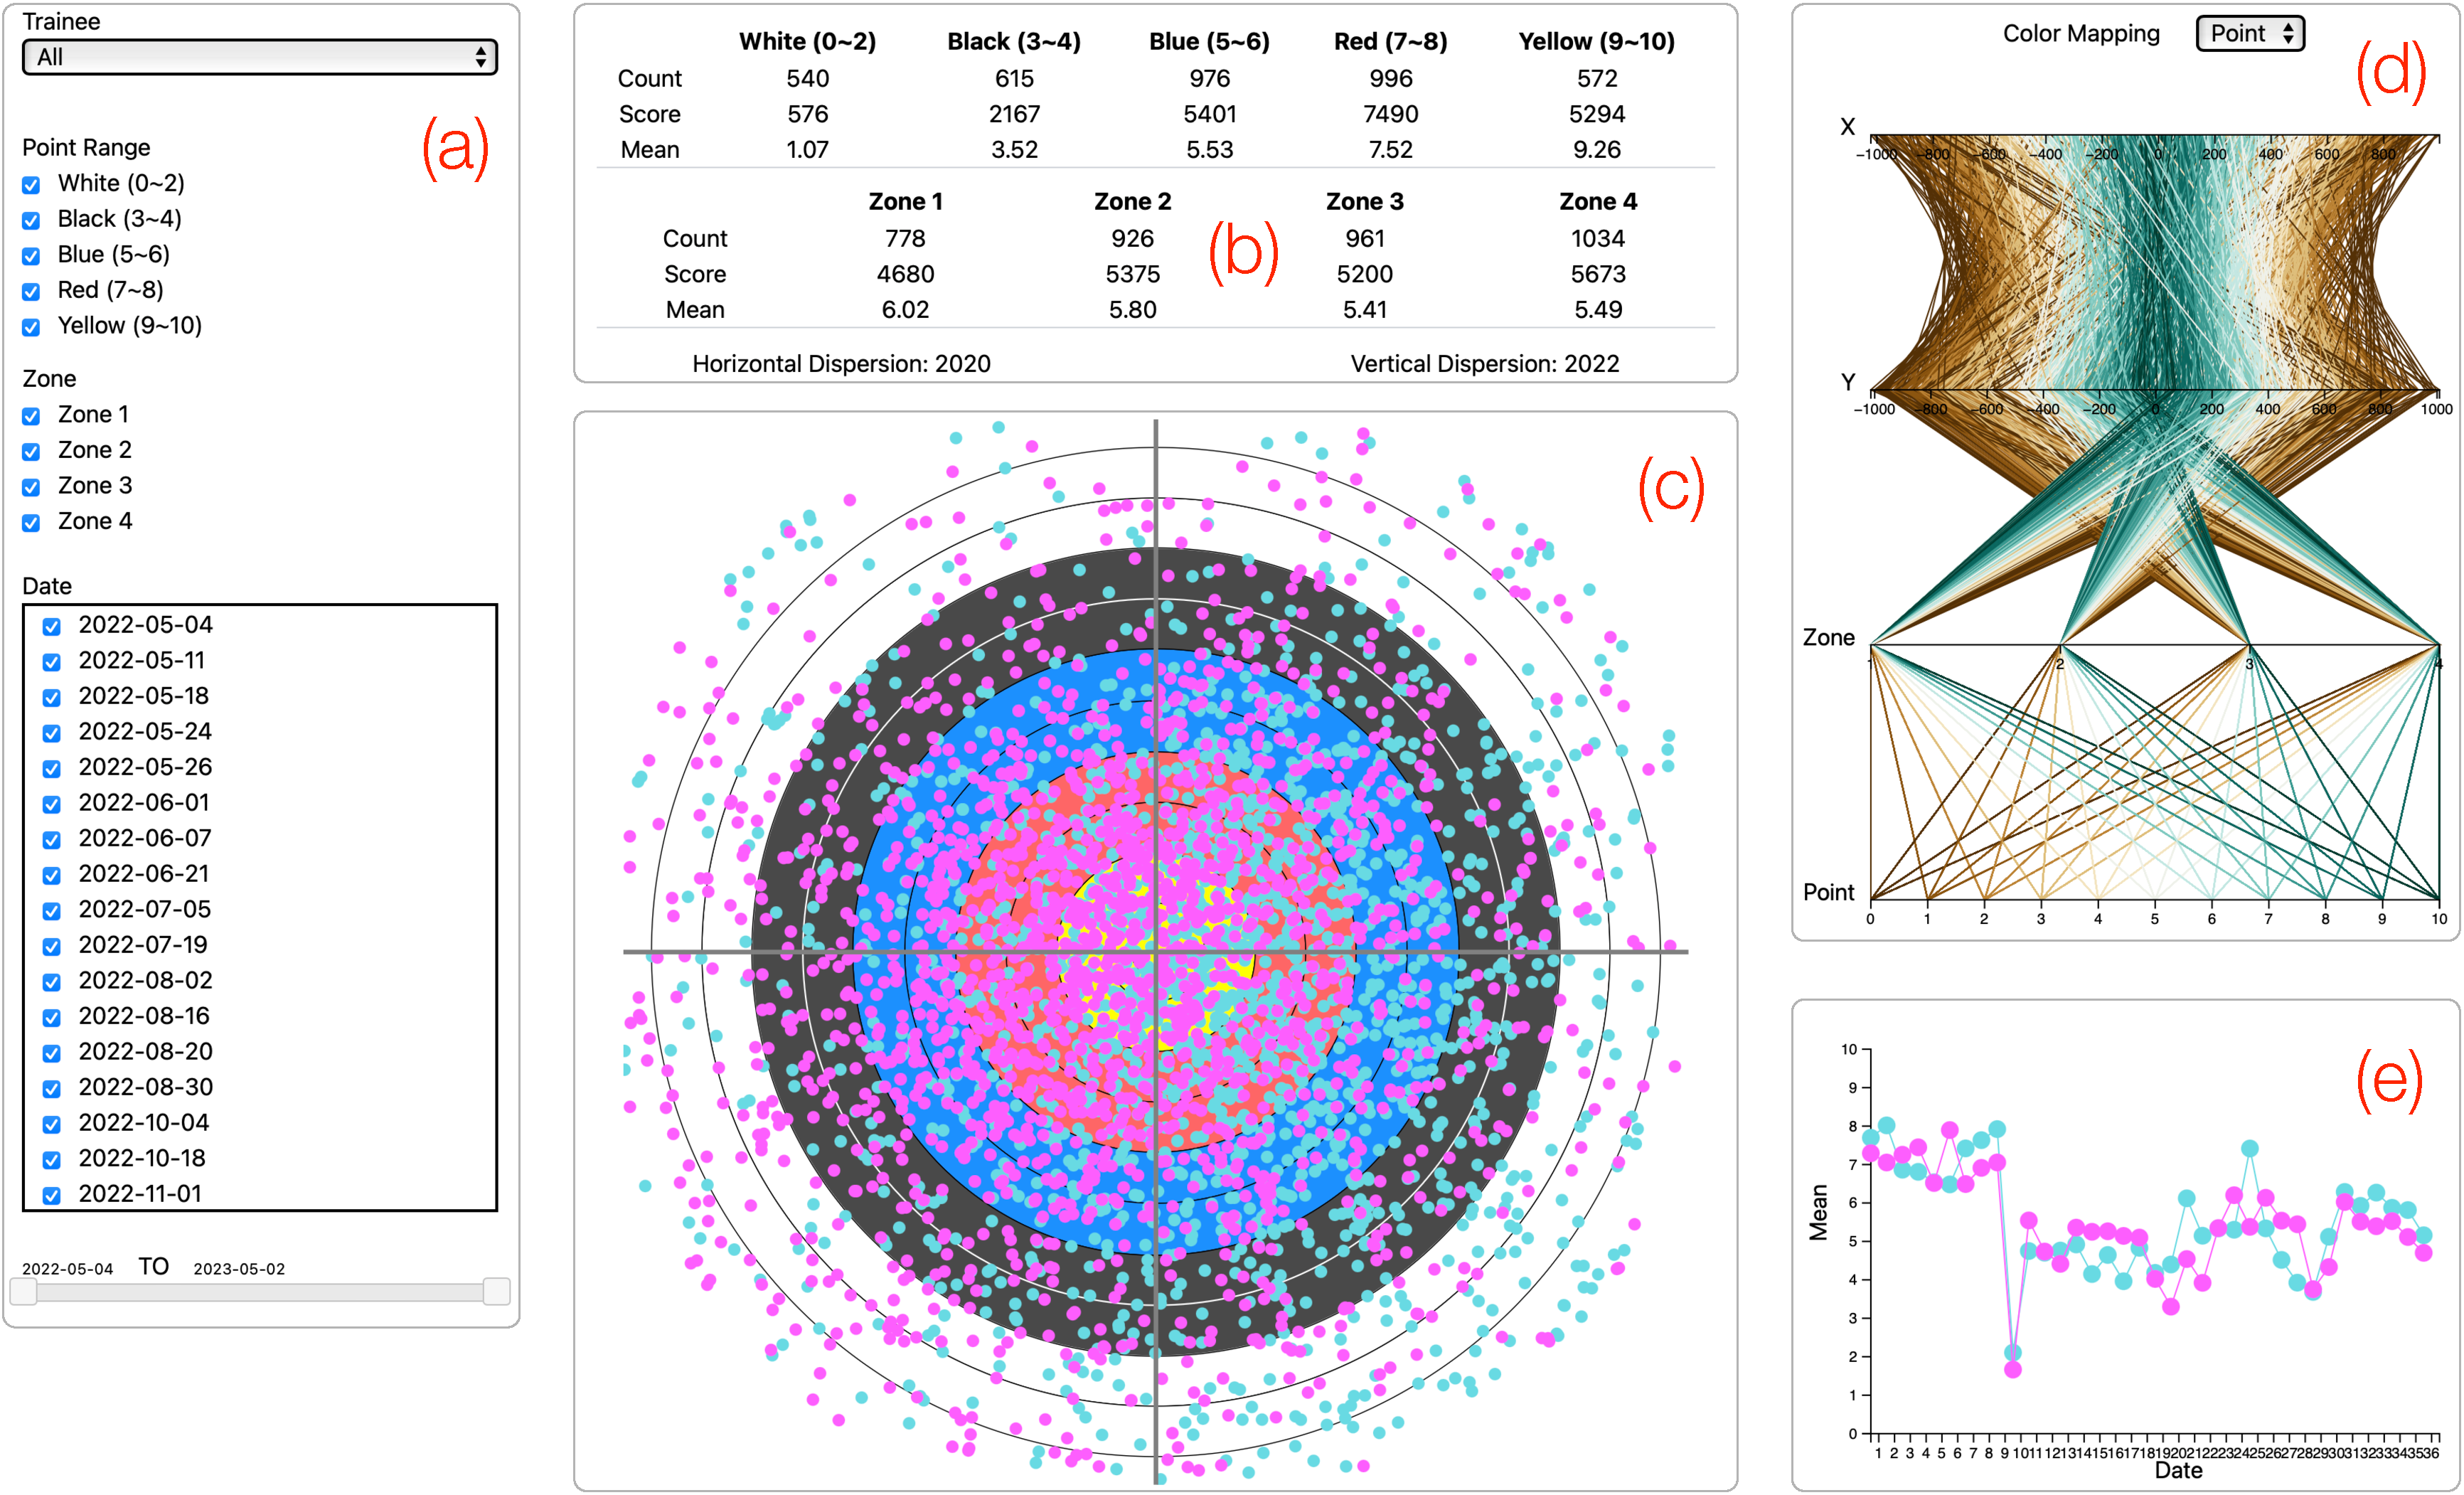
\includegraphics[width=1.0\linewidth]{figures/interface.pdf}
\end{center}
\caption{The ArcheryVis interface consists of (a) multiple controls and (b) statistics, (c) target, (d) attribute, and (e) temporal views. The visualization here considers all shots by both trainees.}
\label{fig:interface}
\end{figure*}

\section{Visual Interface and Interaction}

Figure~\ref{fig:interface} shows a screenshot of the ArcheryVis visual interface, developed using D3~\cite{D3-online}. 
The interface has controls on the left, the primary target view in the middle with the statistics view on its top, and two other views on the right (top-right: attribute view, bottom-right: temporal view).  
%
The controls allow users to choose the trainee(s) and filter shots in the views based on the point range, zone, and date (range). 
The target view reconstructs the shots. The shots of the boy and girl are drawn in cyan and pink colors for differentiation. Mousing over a shot displays a tooltip showing its relevant information (name, $x$-coordinate, $y$-coordinate, date, and point). 
%
The statistics view displays the count, score, and mean across point ranges and zones of displayed or highlighted shots in tabular form. It also reports horizontal and vertical dispersions. 
%Users can toggle heatmap and \hot{???} options to add additional layers providing more visual information. 
%
The attribute view displays shot data using parallel coordinates along four dimensions: $x$-coordinate, $y$-coordinate, zone, and point. Users can color each shot (displayed as a polyline) in this view based on a chosen dimension. They can also brush one or more dimensions for filtering. 
%
Finally, the temporal view plots the performance over dates using the mean value. Mousing over a date displays a tooltip with relevant information (date, count, score, mean, and standard deviation) and highlights the corresponding shots in the target view. 

%covariance ellipse~\cite{Schelp-online} showing the spread and directionality of the shots

\begin{figure*}[htb]
\begin{center}
$\begin{array}{c@{\hspace{0.025in}}c@{\hspace{0.025in}}c@{\hspace{0.025in}}c}
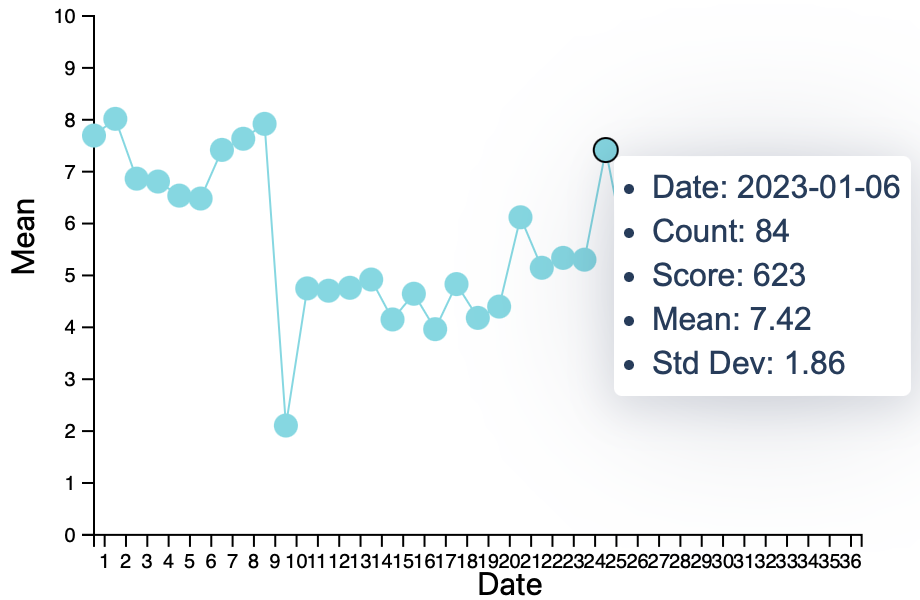
\includegraphics[height=0.75in]{figures/brushing-target-temporal-2.png}&
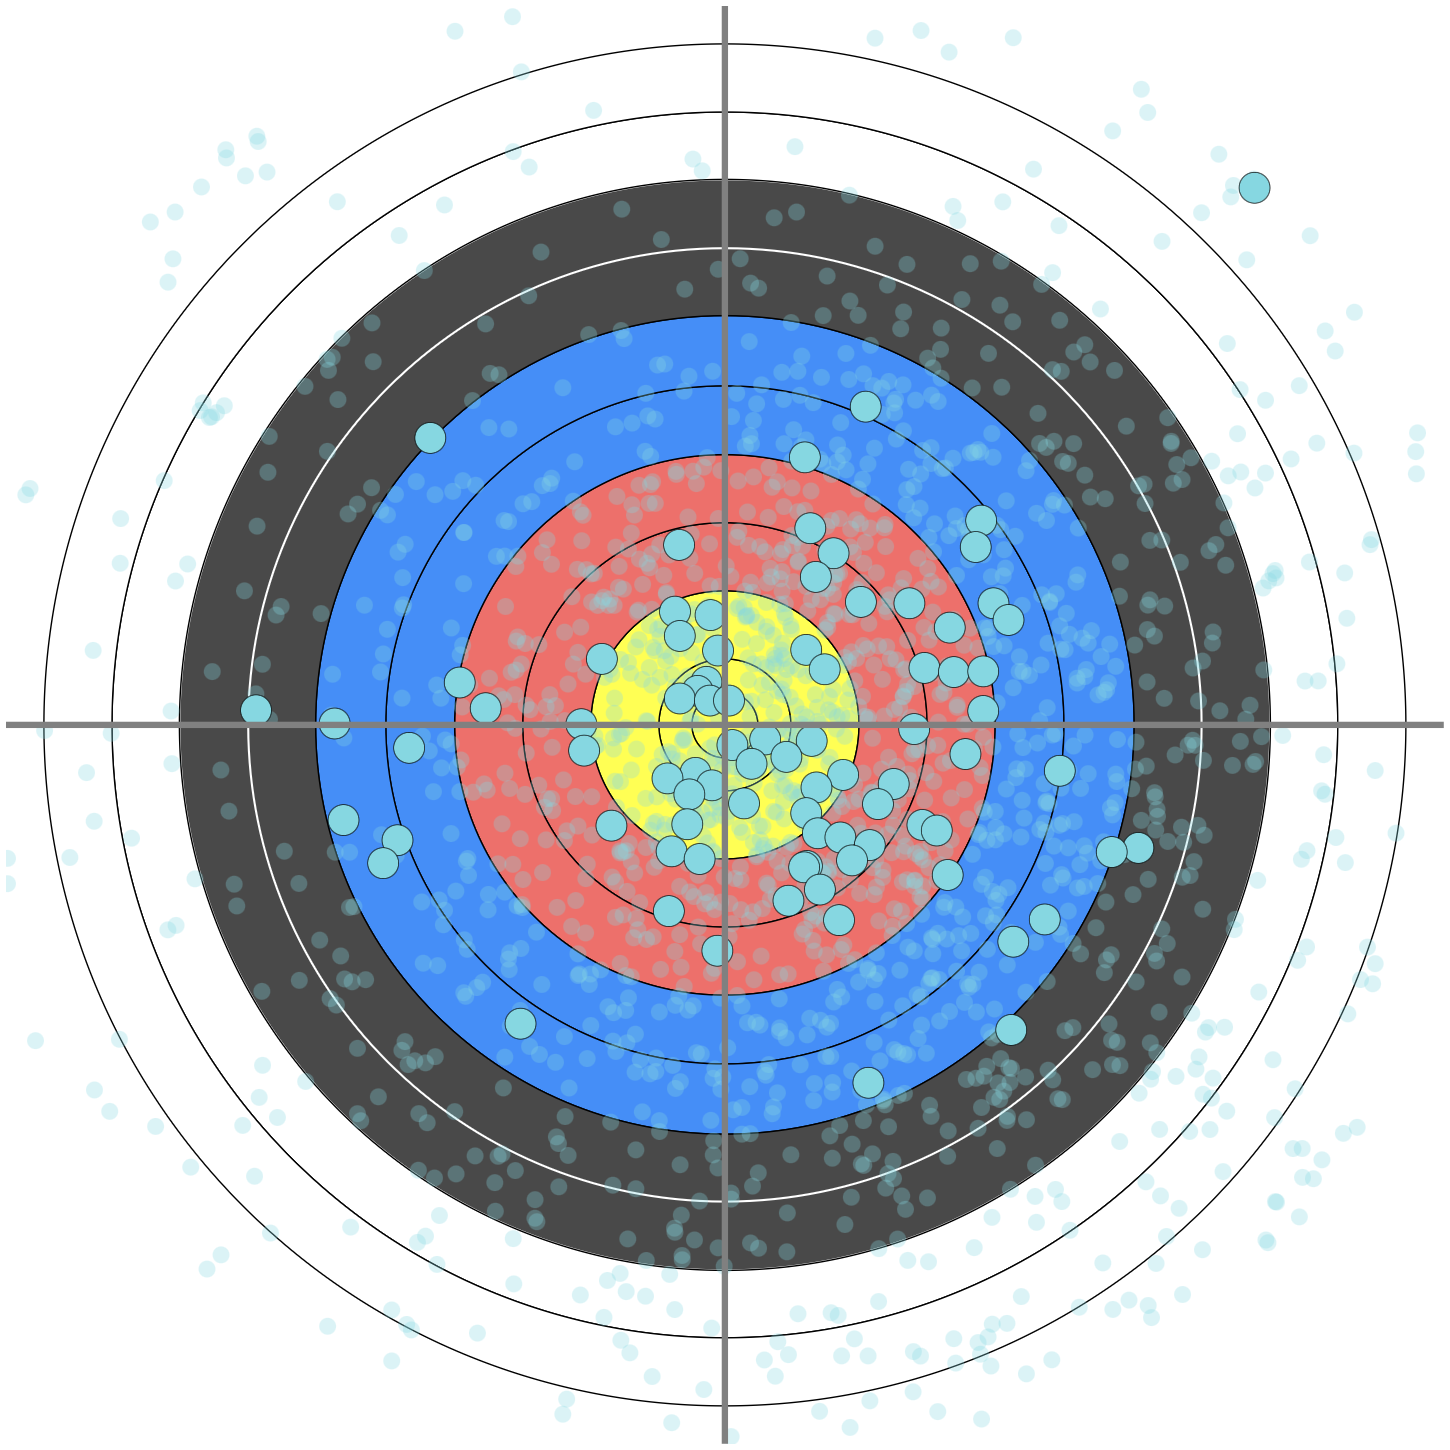
\includegraphics[height=1.25in]{figures/brushing-target-temporal-1.png}&
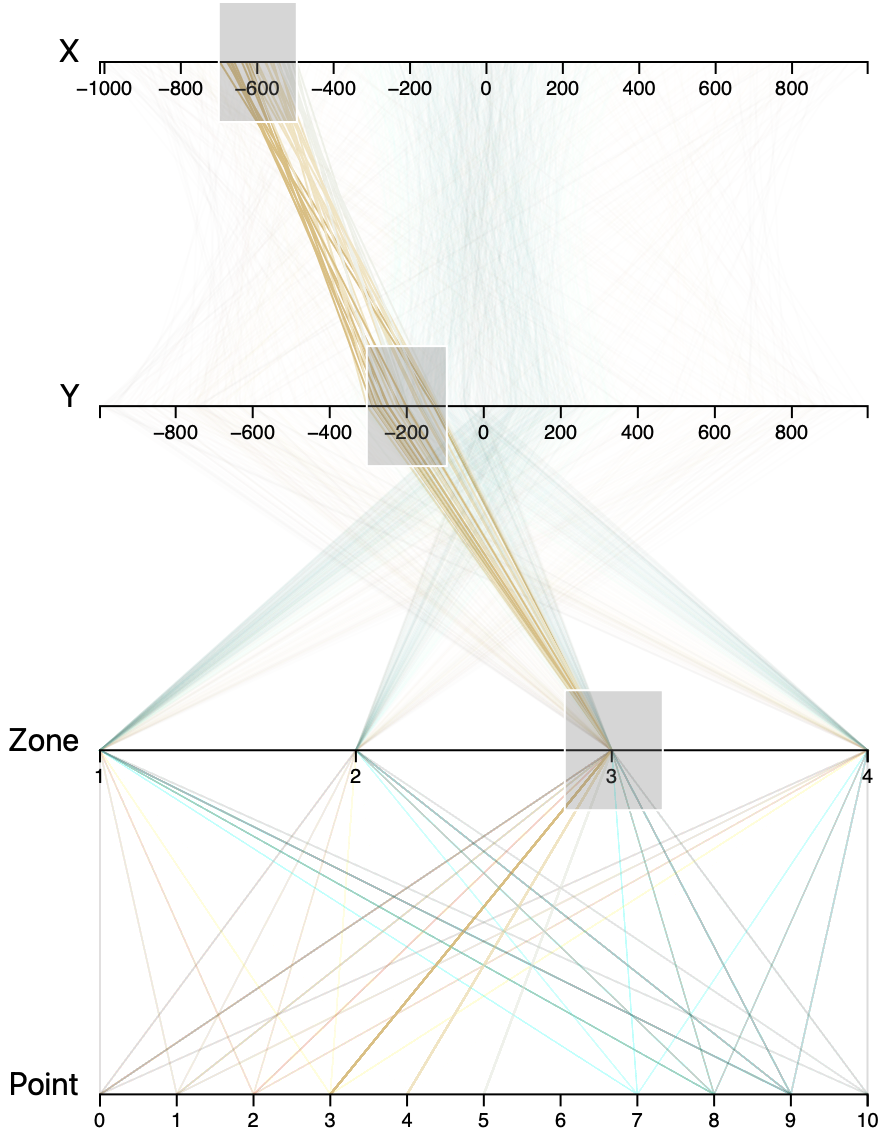
\includegraphics[height=1.25in]{figures/brushing-target-attribute-2.png}&
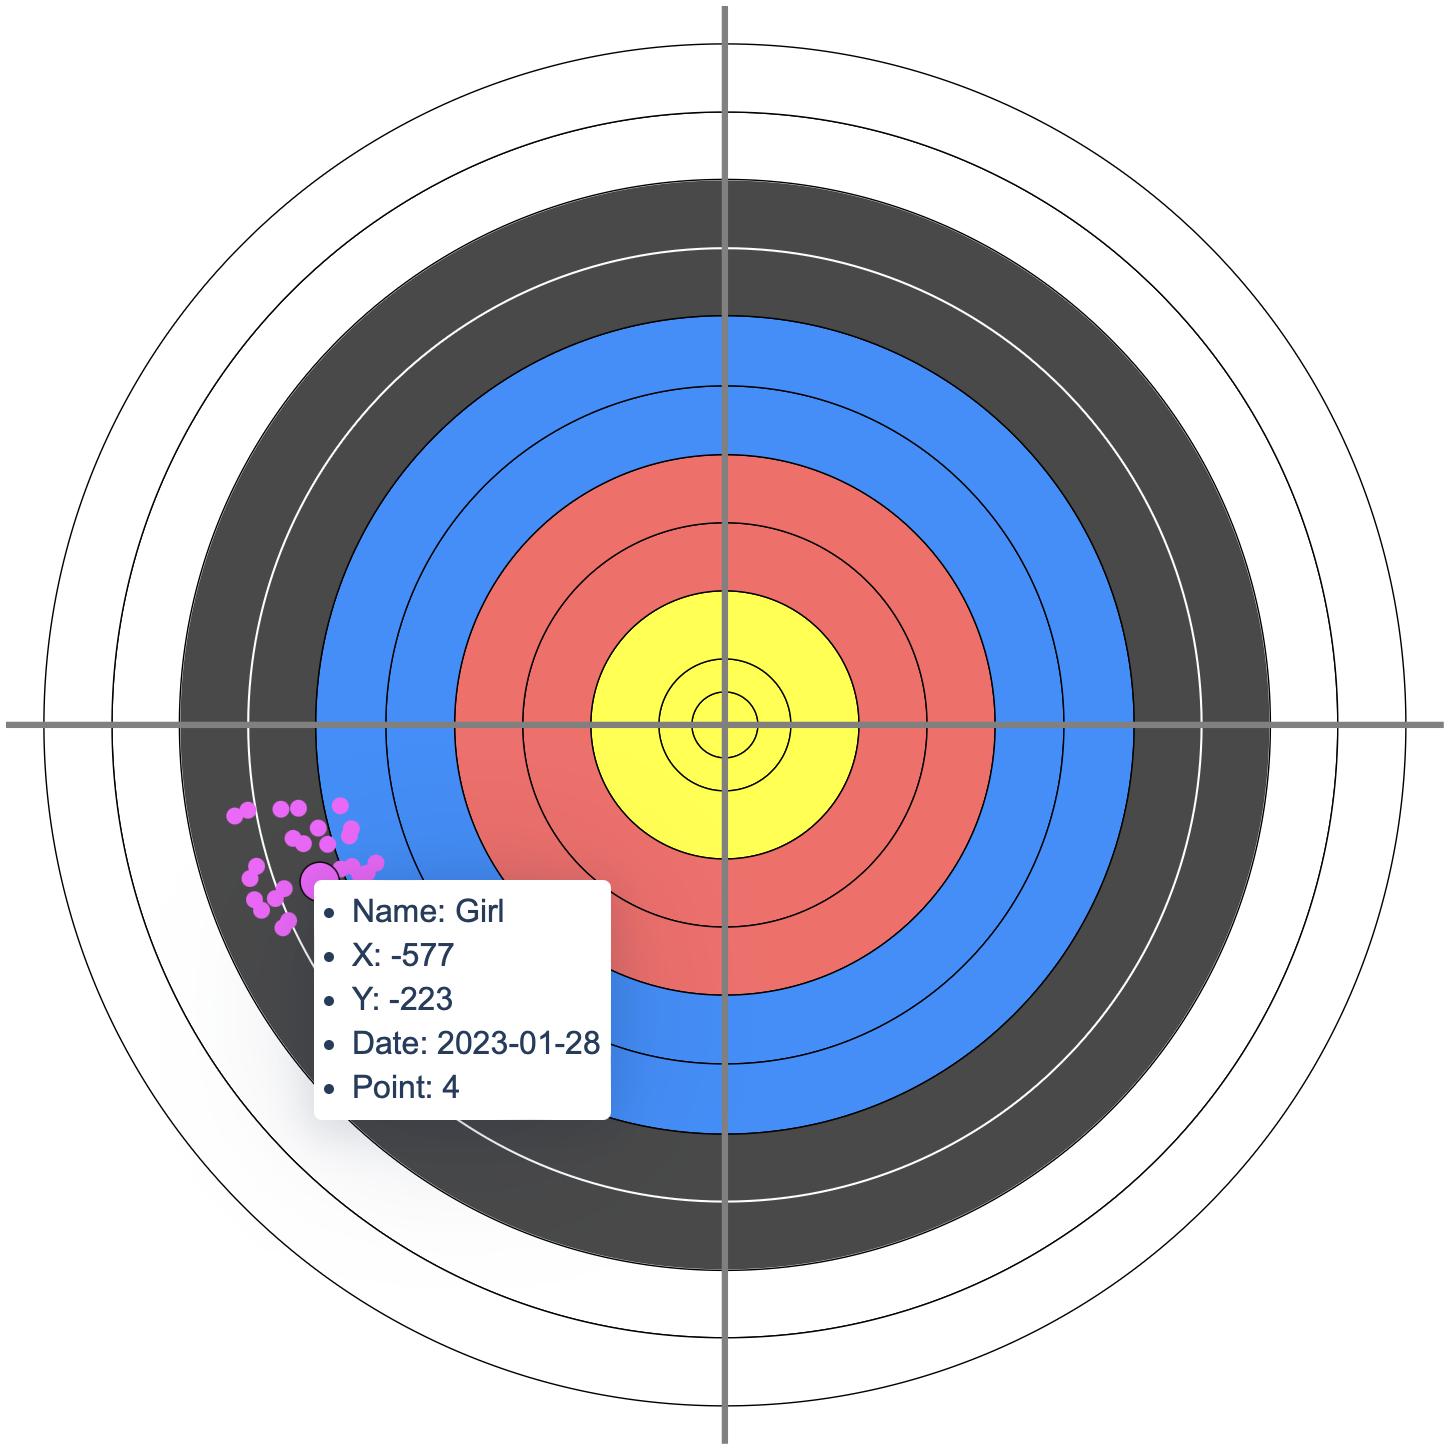
\includegraphics[height=1.25in]{figures/brushing-target-attribute-1.png}\\
\mbox{(a)} & \mbox{(b)} & \mbox{(c)} & \mbox{(d)}
\end{array}$
\end{center}
\caption{Two examples of brushing and linking. Brushing (a) the temporal view links to (b) the target view. Brushing (c) the attribute view links to (d) the target view.}
\label{fig:brushing}
\end{figure*}

\begin{figure*}[htb]
\begin{center}
$\begin{array}{c@{\hspace{0.05in}}c@{\hspace{0.05in}}c@{\hspace{0.05in}}c}
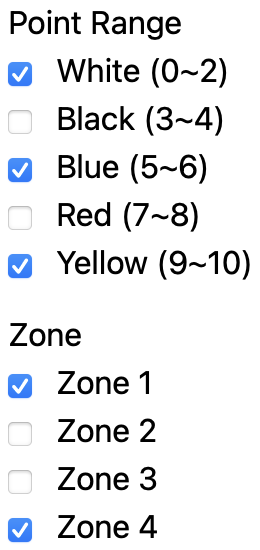
\includegraphics[width=0.08\linewidth]{figures/filter-controls-range-zone-2.png}&
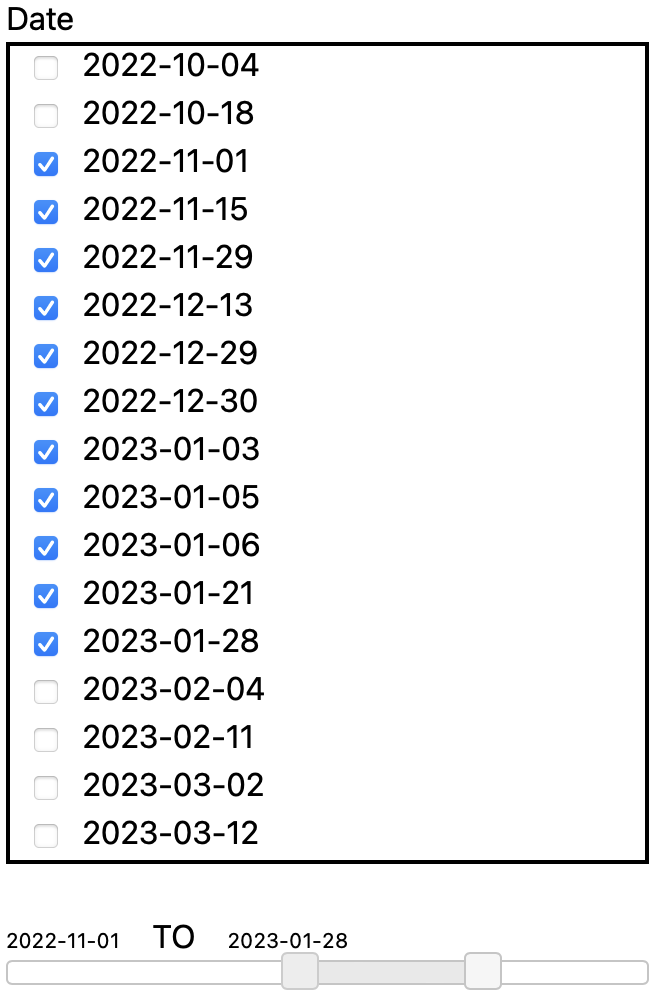
\includegraphics[width=0.185\linewidth]{figures/filter-controls-date-2.png}&
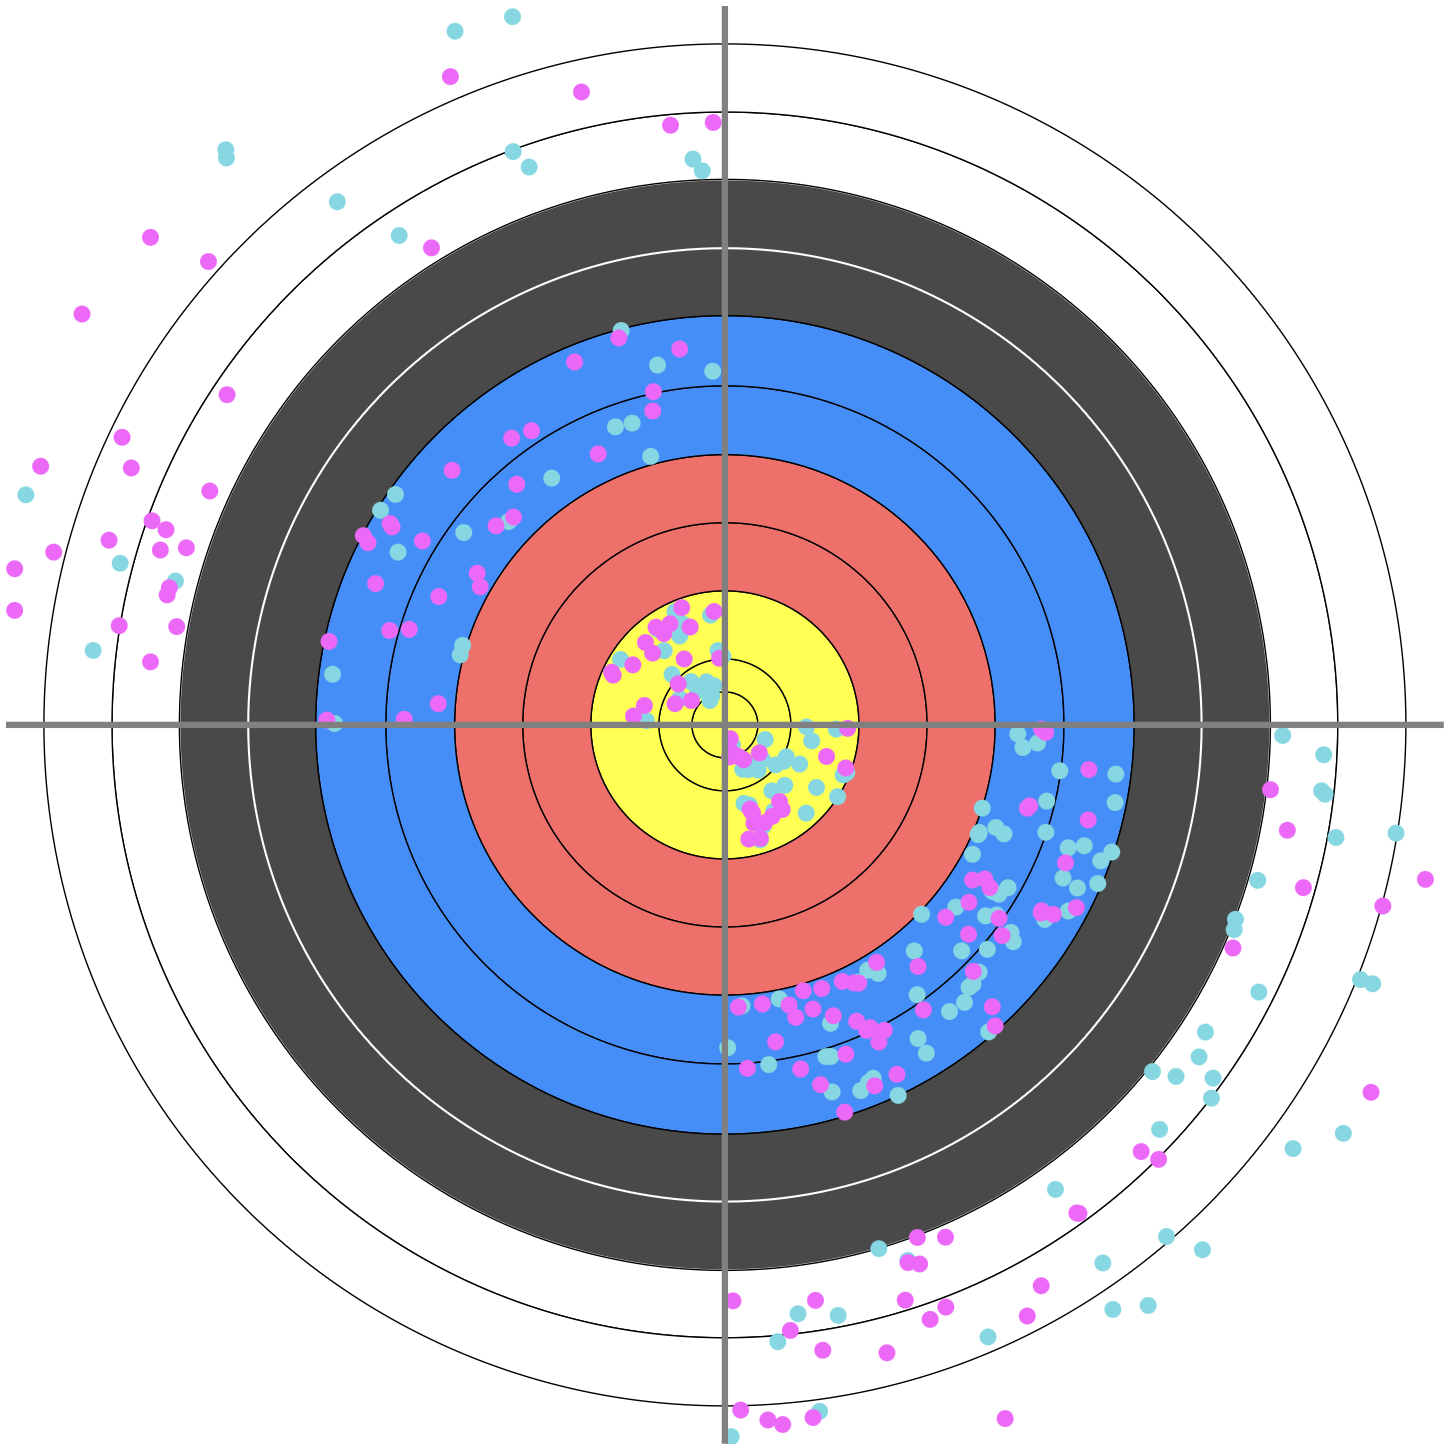
\includegraphics[height=1.35in]{figures/filter-controls-target-2.png}&
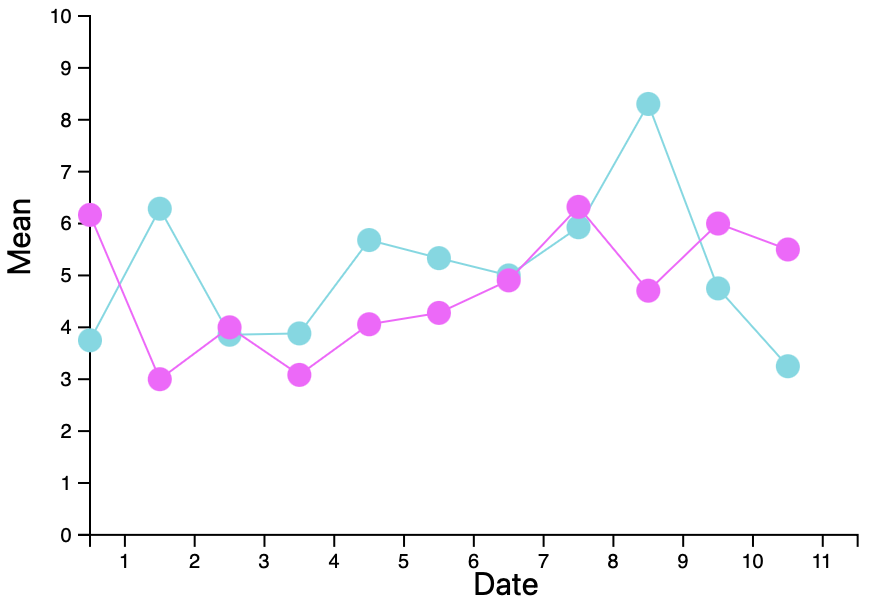
\includegraphics[height=0.85in]{figures/filter-controls-temporal-2.png}\\
\mbox{(a)} & \mbox{(b)} & \mbox{(c)} & \mbox{(d)}
\end{array}$
\end{center}
\caption{An example of filtering using controls of (a) point range and zone, and (b) date (range). (c) and (d) show the resulting target and temporal views.}
\label{fig:filtering-2}
\end{figure*}

\begin{figure*}[htb]
\begin{center}
$\begin{array}{c@{\hspace{0.025in}}c@{\hspace{0.025in}}c@{\hspace{0.025in}}c}
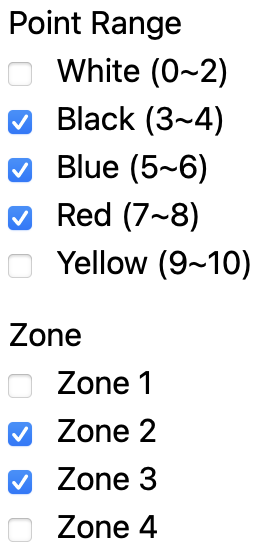
\includegraphics[width=0.08\linewidth]{figures/filter-controls-range-zone-1.png}&
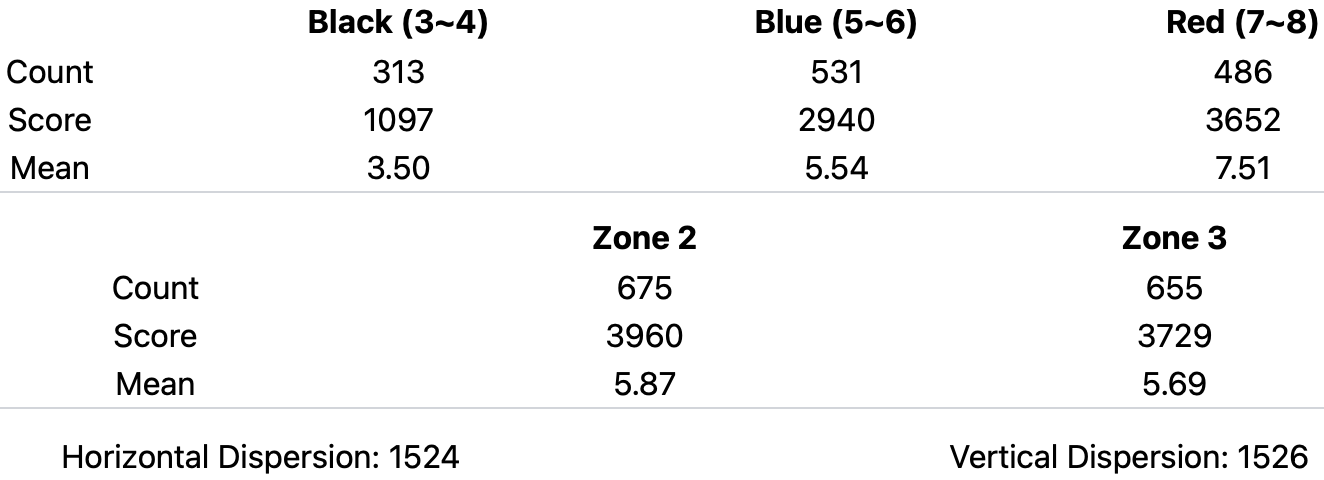
\includegraphics[width=0.375\linewidth]{figures/filter-controls-statistics-1.png}&
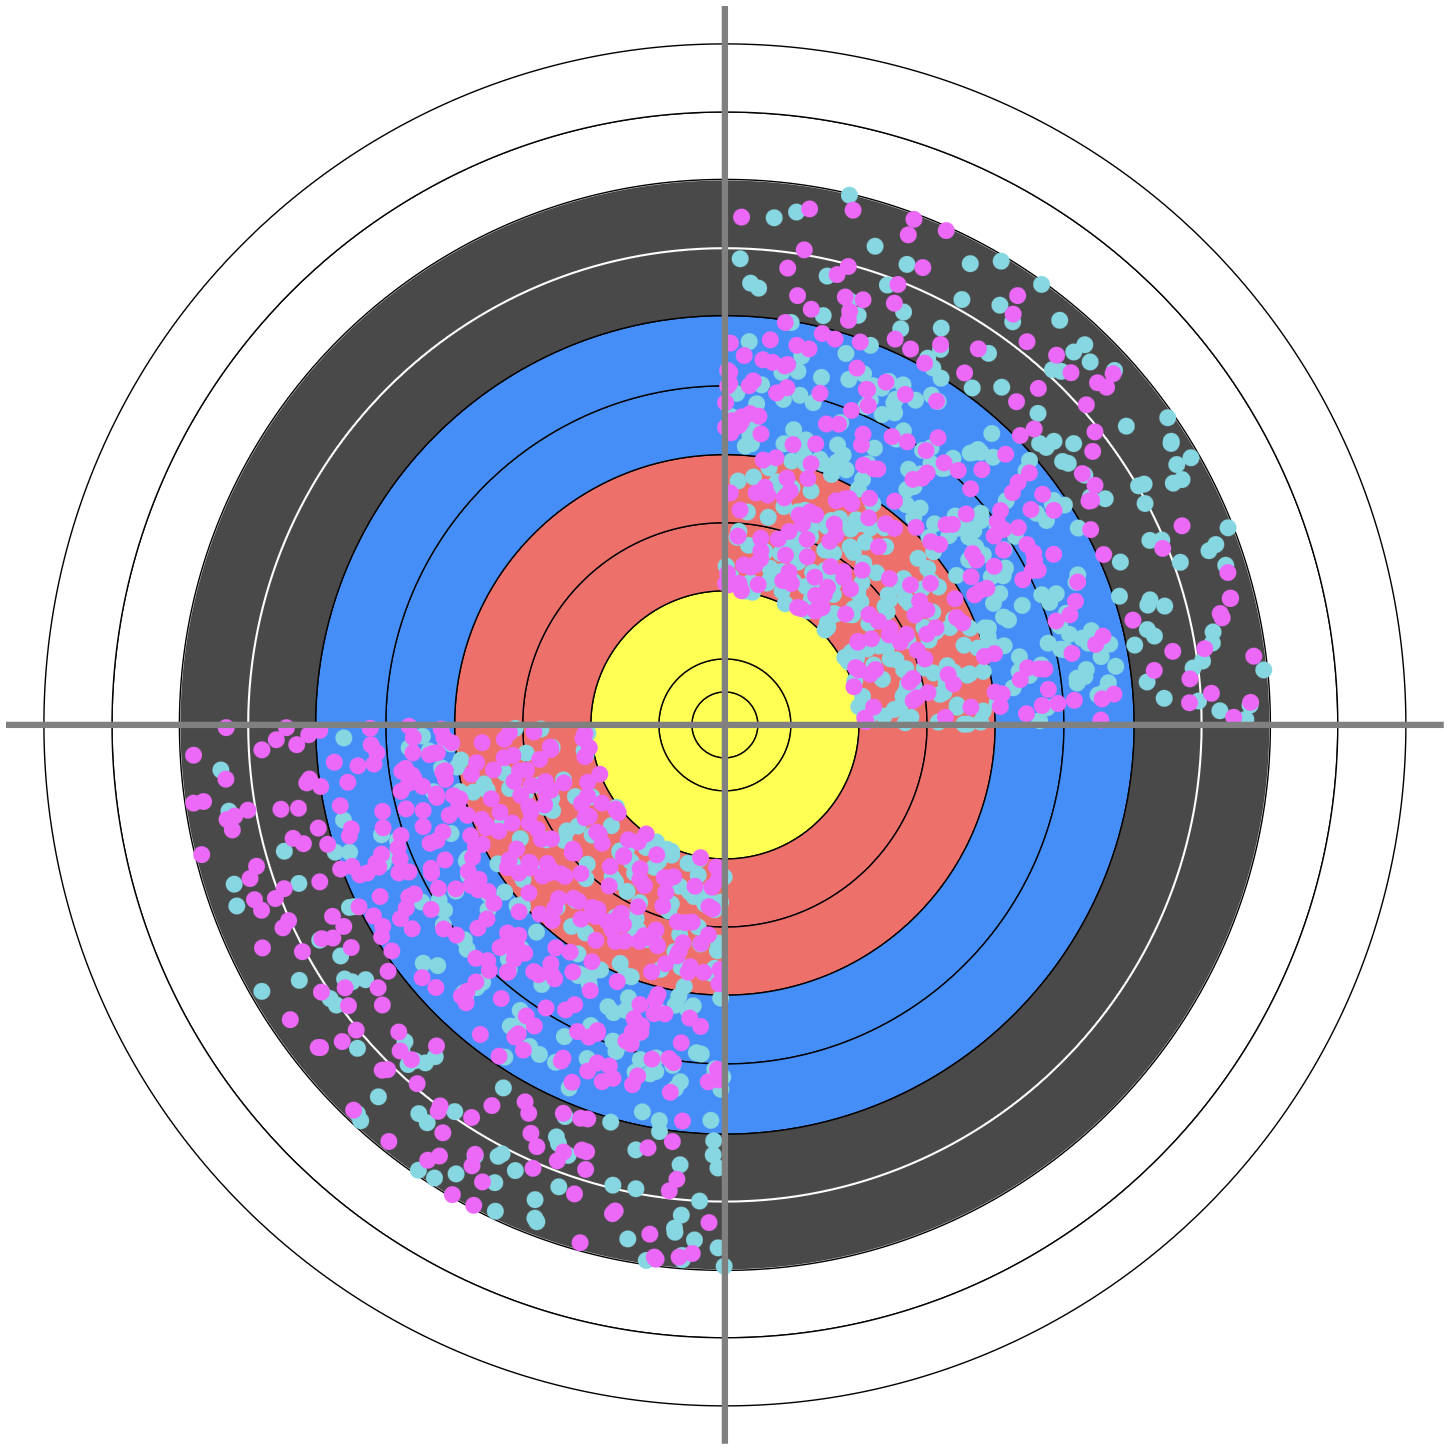
\includegraphics[height=1.25in]{figures/filter-controls-target-1.png}&
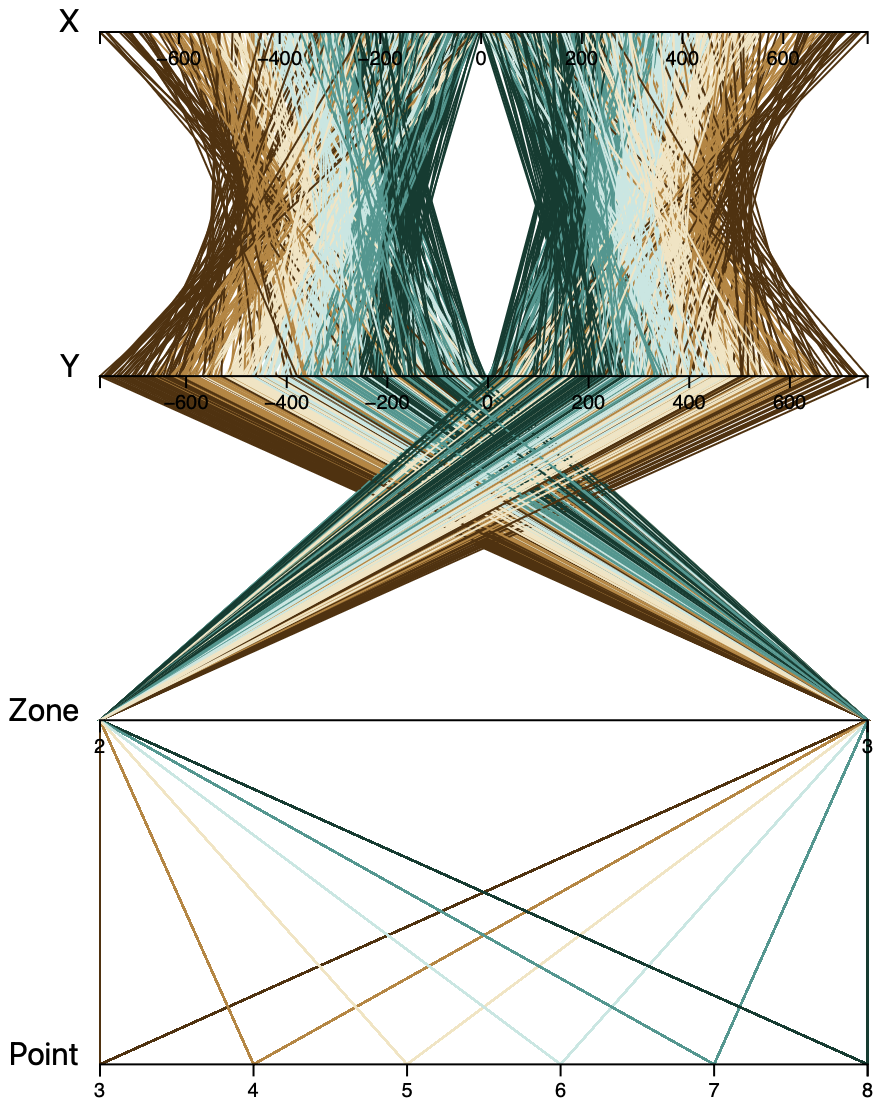
\includegraphics[height=1.25in]{figures/filter-controls-attribute-1.png}\\
\mbox{(a)} & \mbox{(b)} & \mbox{(c)} & \mbox{(d)}
\end{array}$
\end{center}
\caption{Another filtering example using controls of (a) point range and zone. (b) to (d) show the resulting statistics, target, and attribute views.}
\label{fig:filtering-1}
\end{figure*}

\begin{figure*}[htb]
\begin{center}
$\begin{array}{c@{\hspace{0.25in}}c}
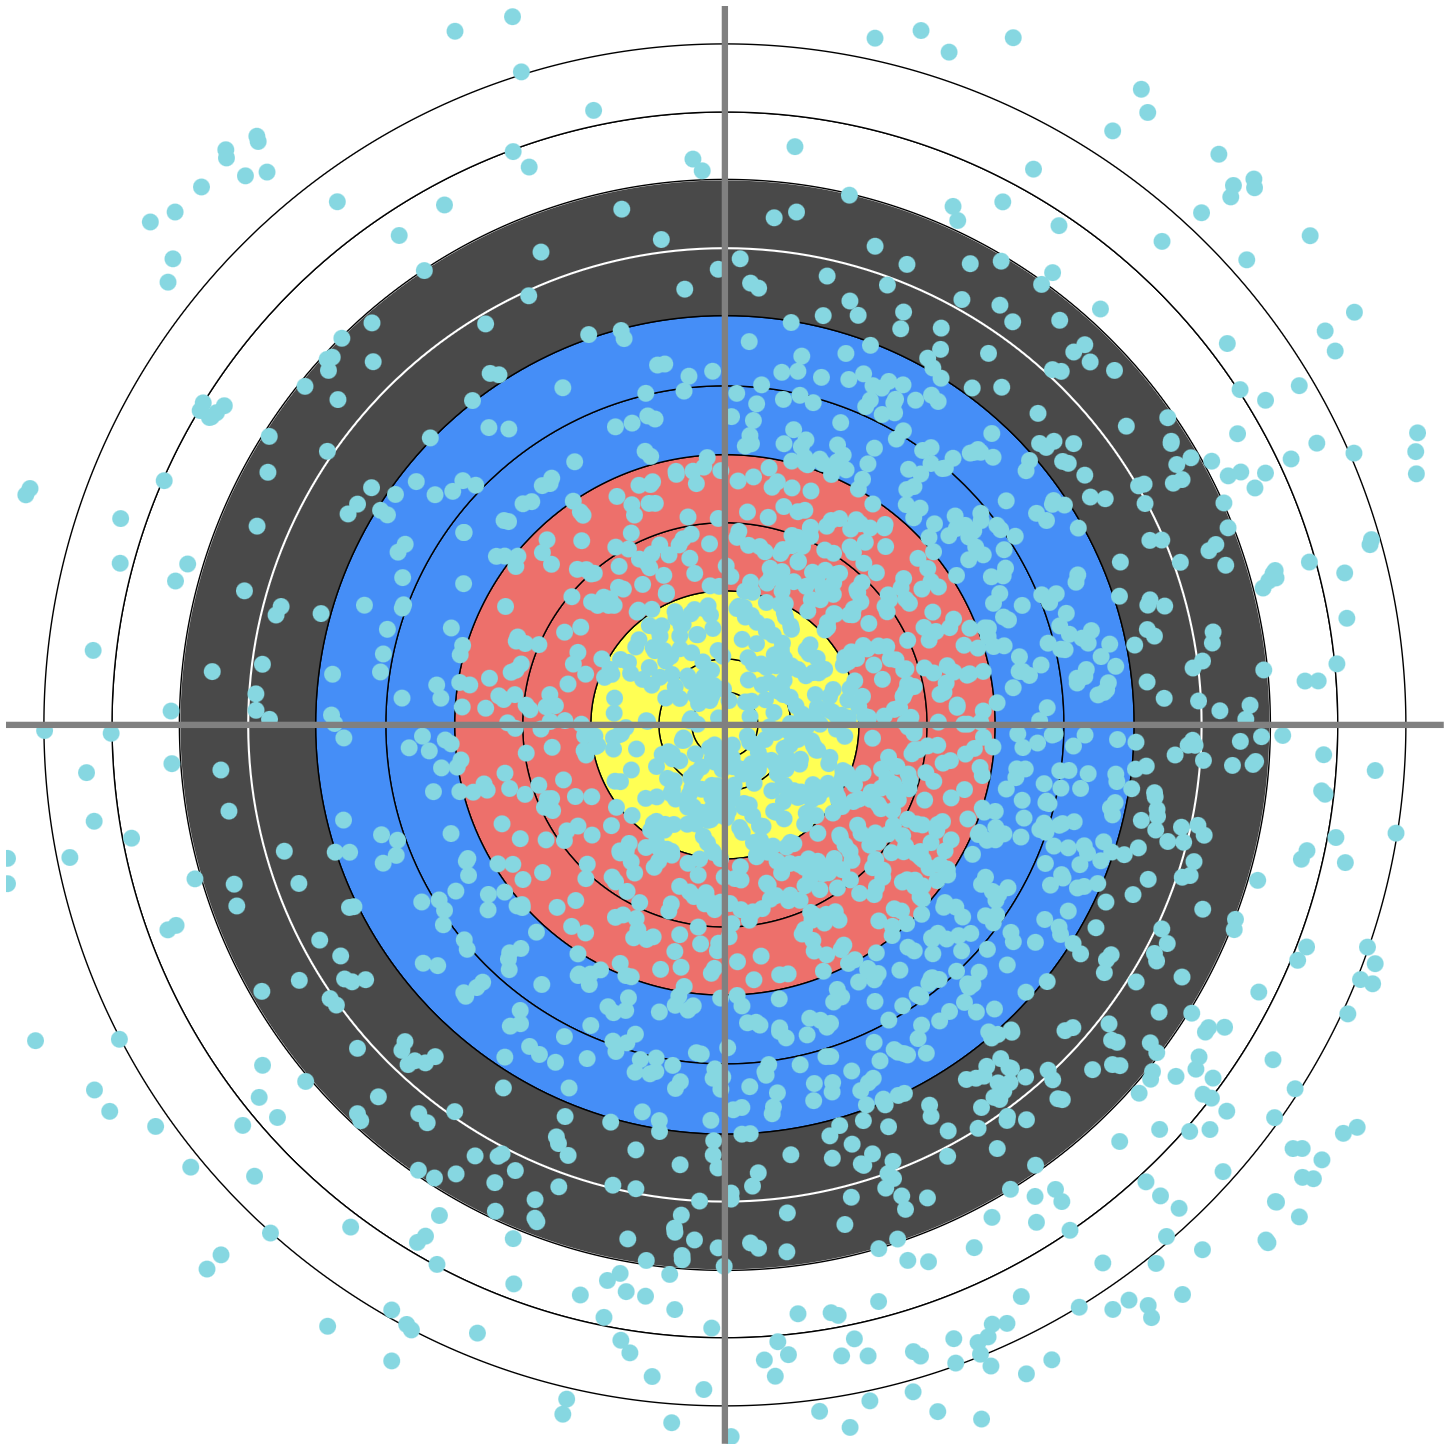
\includegraphics[height=1.75in]{figures/overall-target-boy.png}&
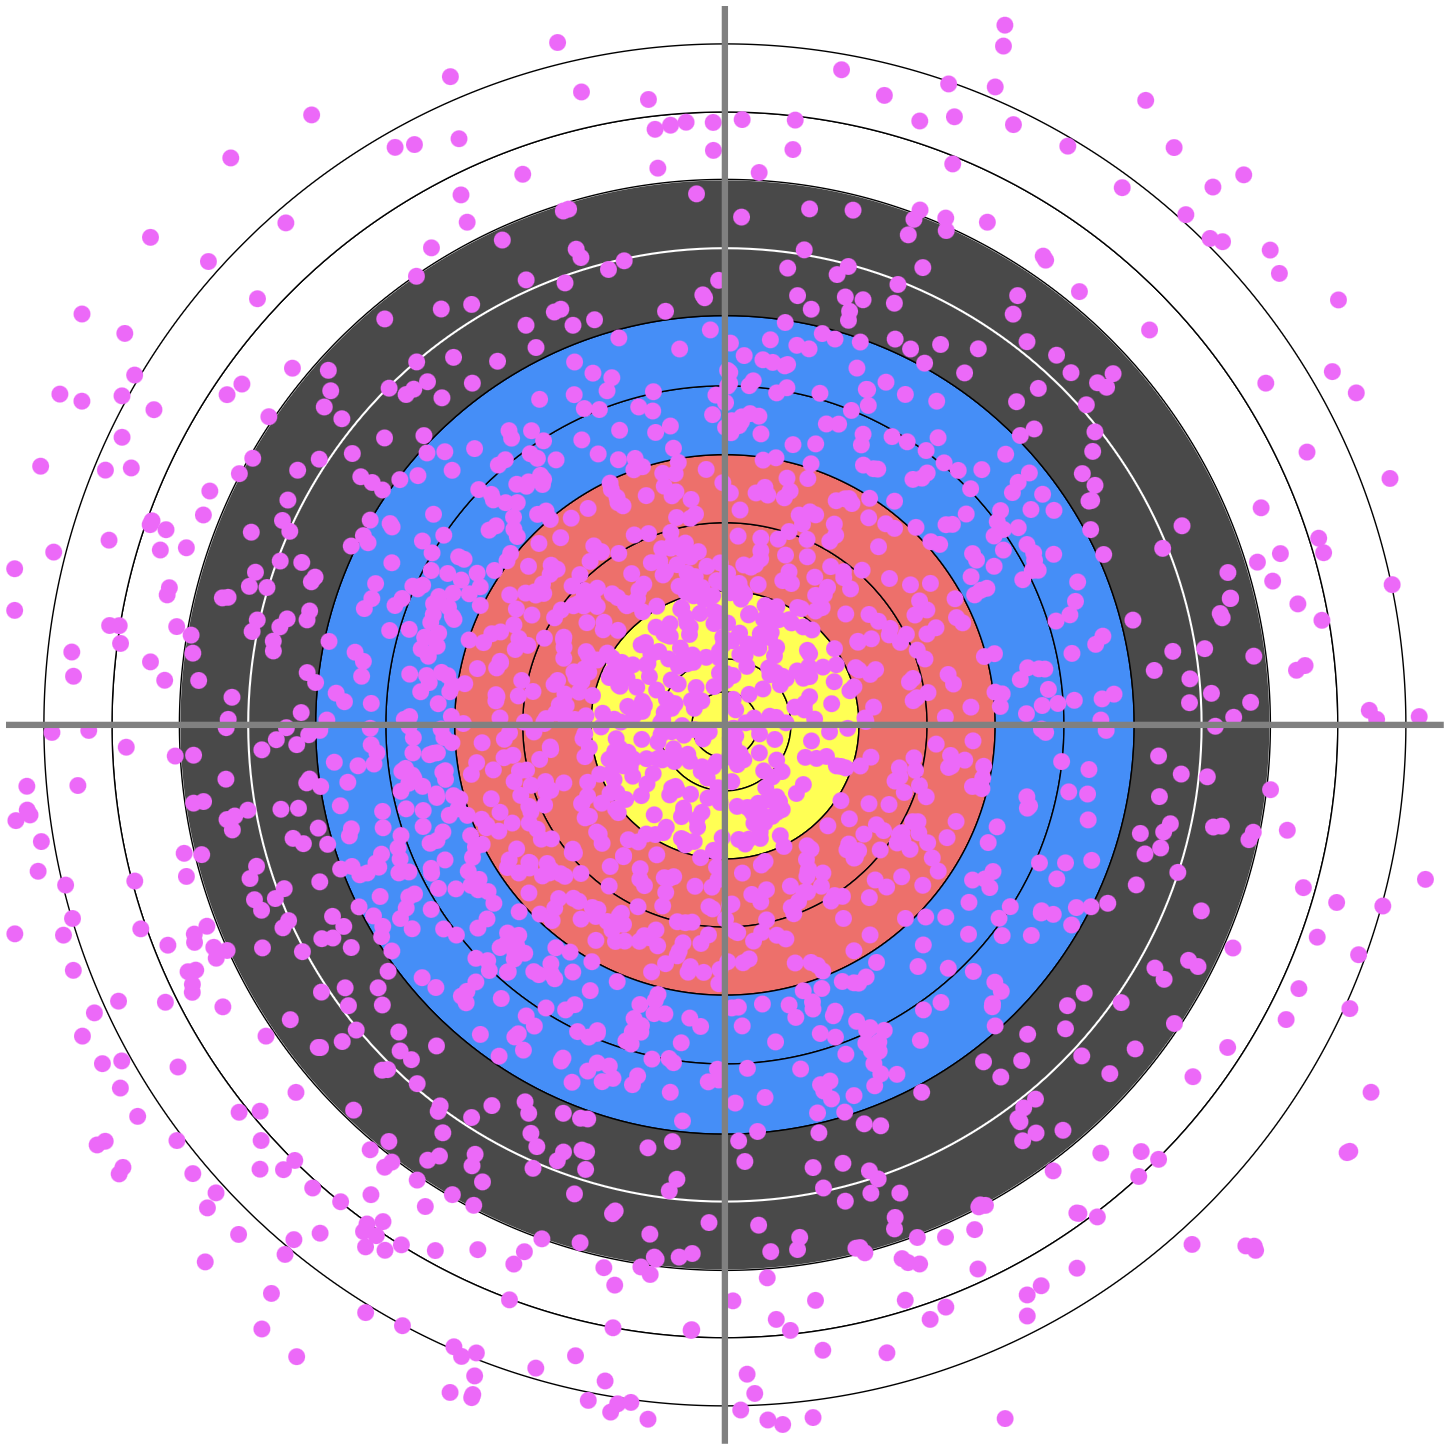
\includegraphics[height=1.75in]{figures/overall-target-girl.png}\\
\mbox{(a)} & \mbox{(b)}
\end{array}$
\end{center}
\caption{The target views of (a) the boy and (b) the girl accumulated over the 36 dates.}
\label{fig:overall-target}
\end{figure*}

\begin{figure*}[htb]
\begin{center}
$\begin{array}{c@{\hspace{0.025in}}c@{\hspace{0.025in}}c@{\hspace{0.025in}}c@{\hspace{0.025in}}c}
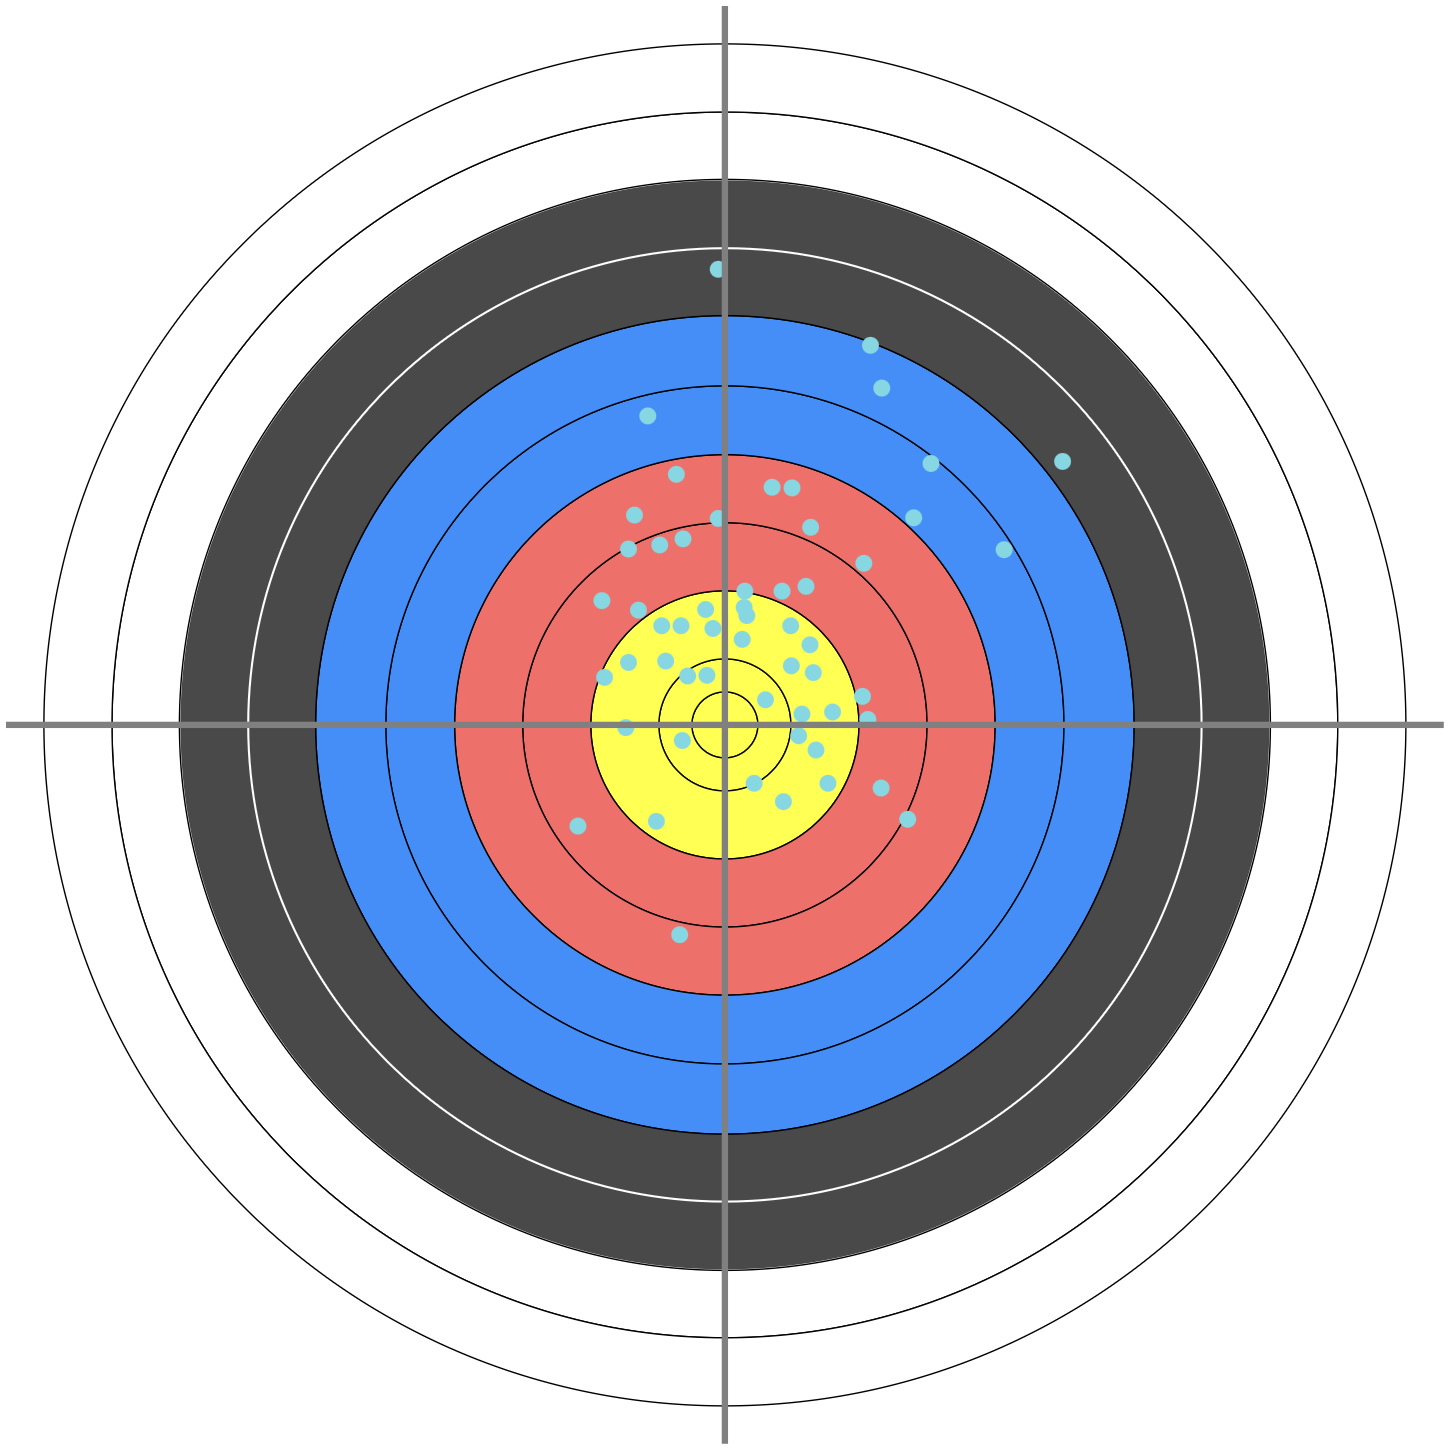
\includegraphics[height=0.825in]{figures/best-date-boy.png}&
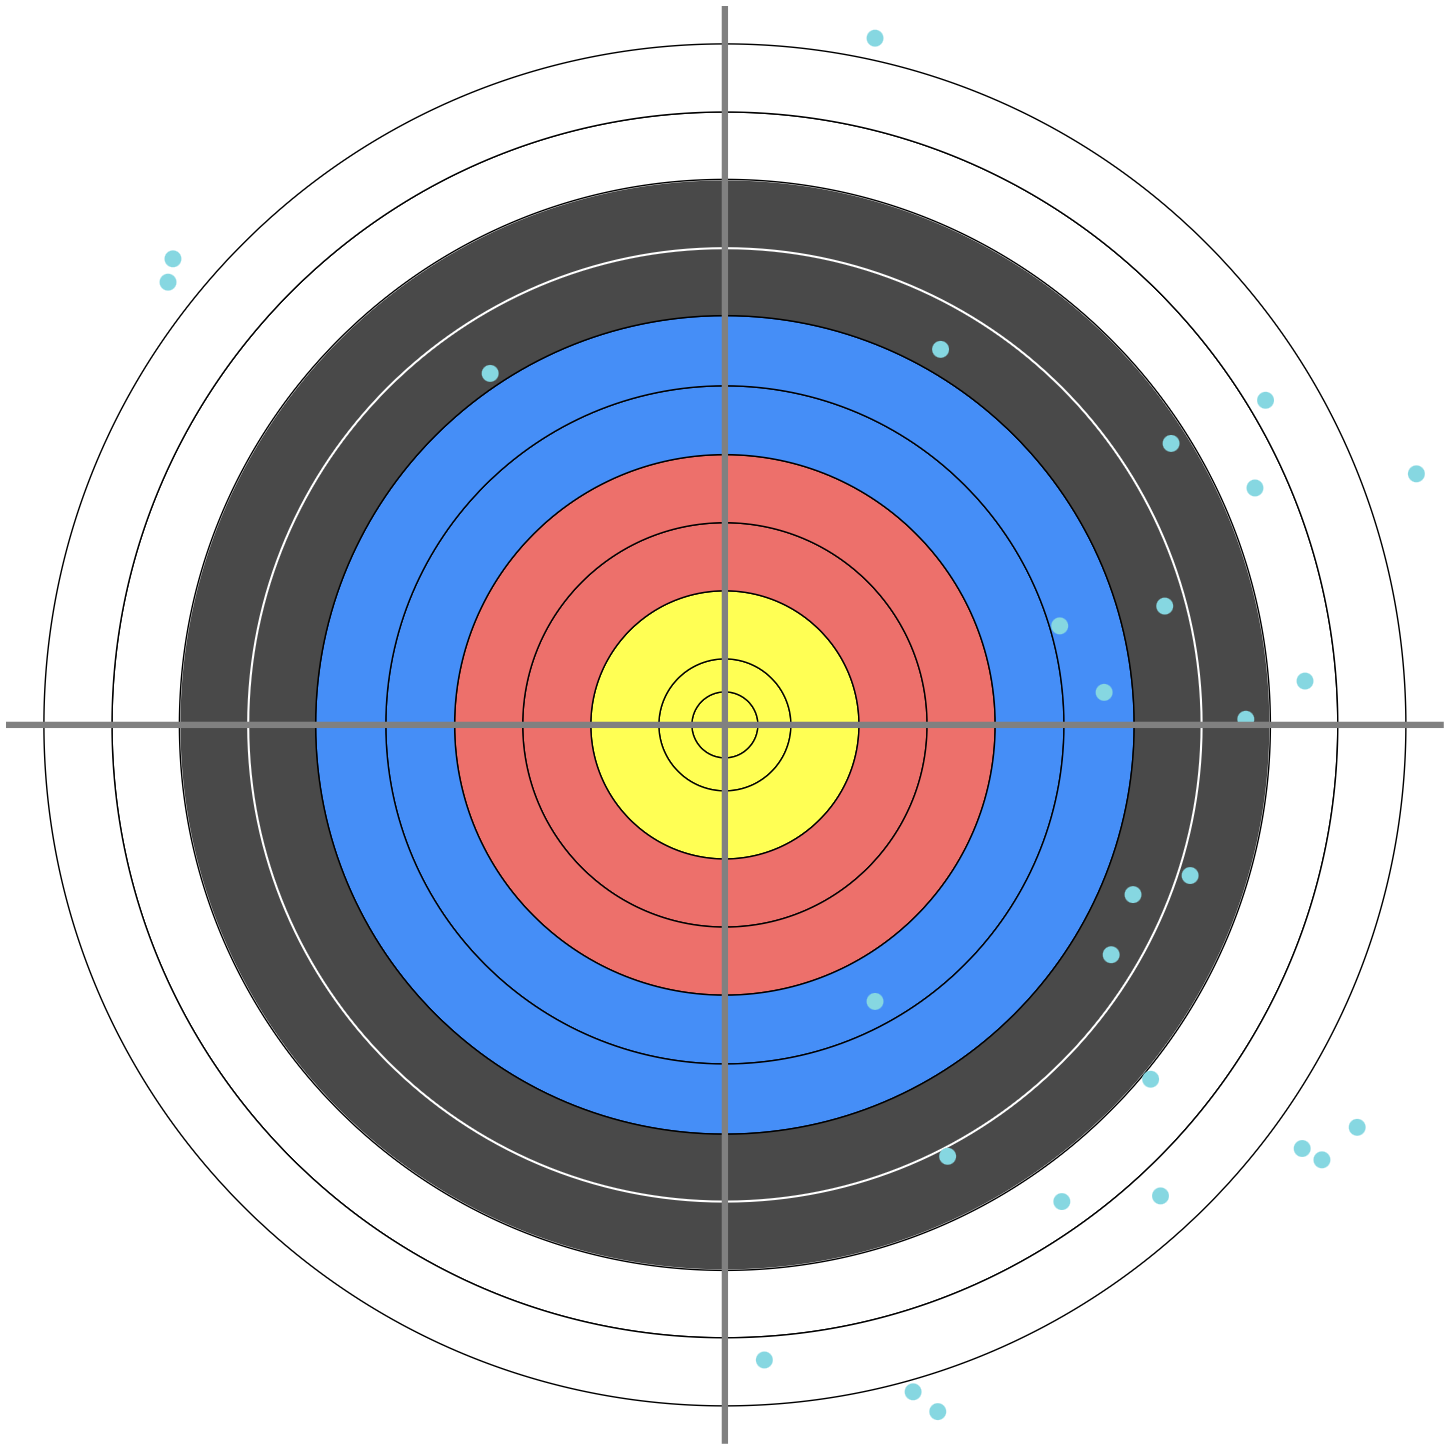
\includegraphics[height=0.825in]{figures/worst-date-boy.png}&
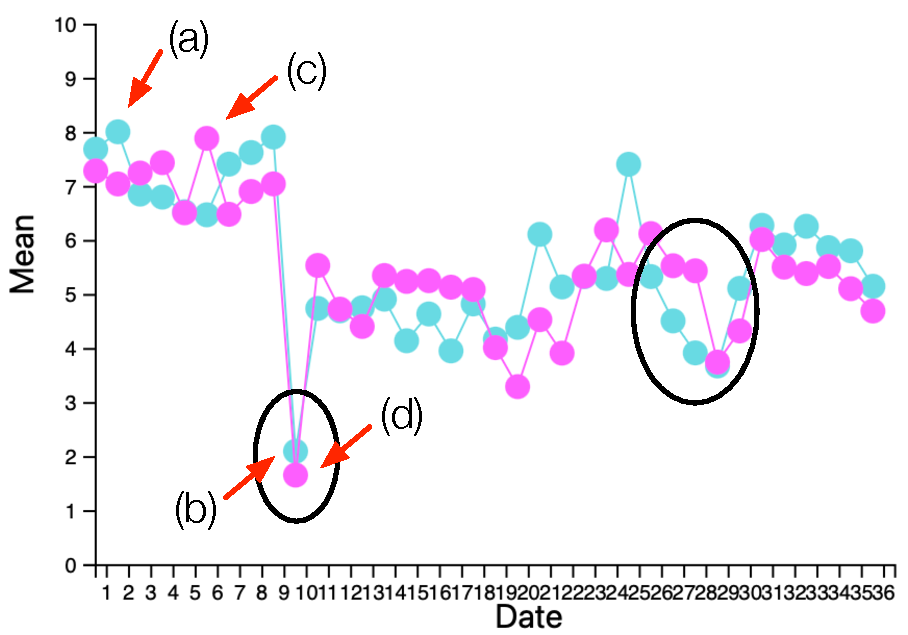
\includegraphics[height=0.825in]{figures/best-worst-dates.pdf}&
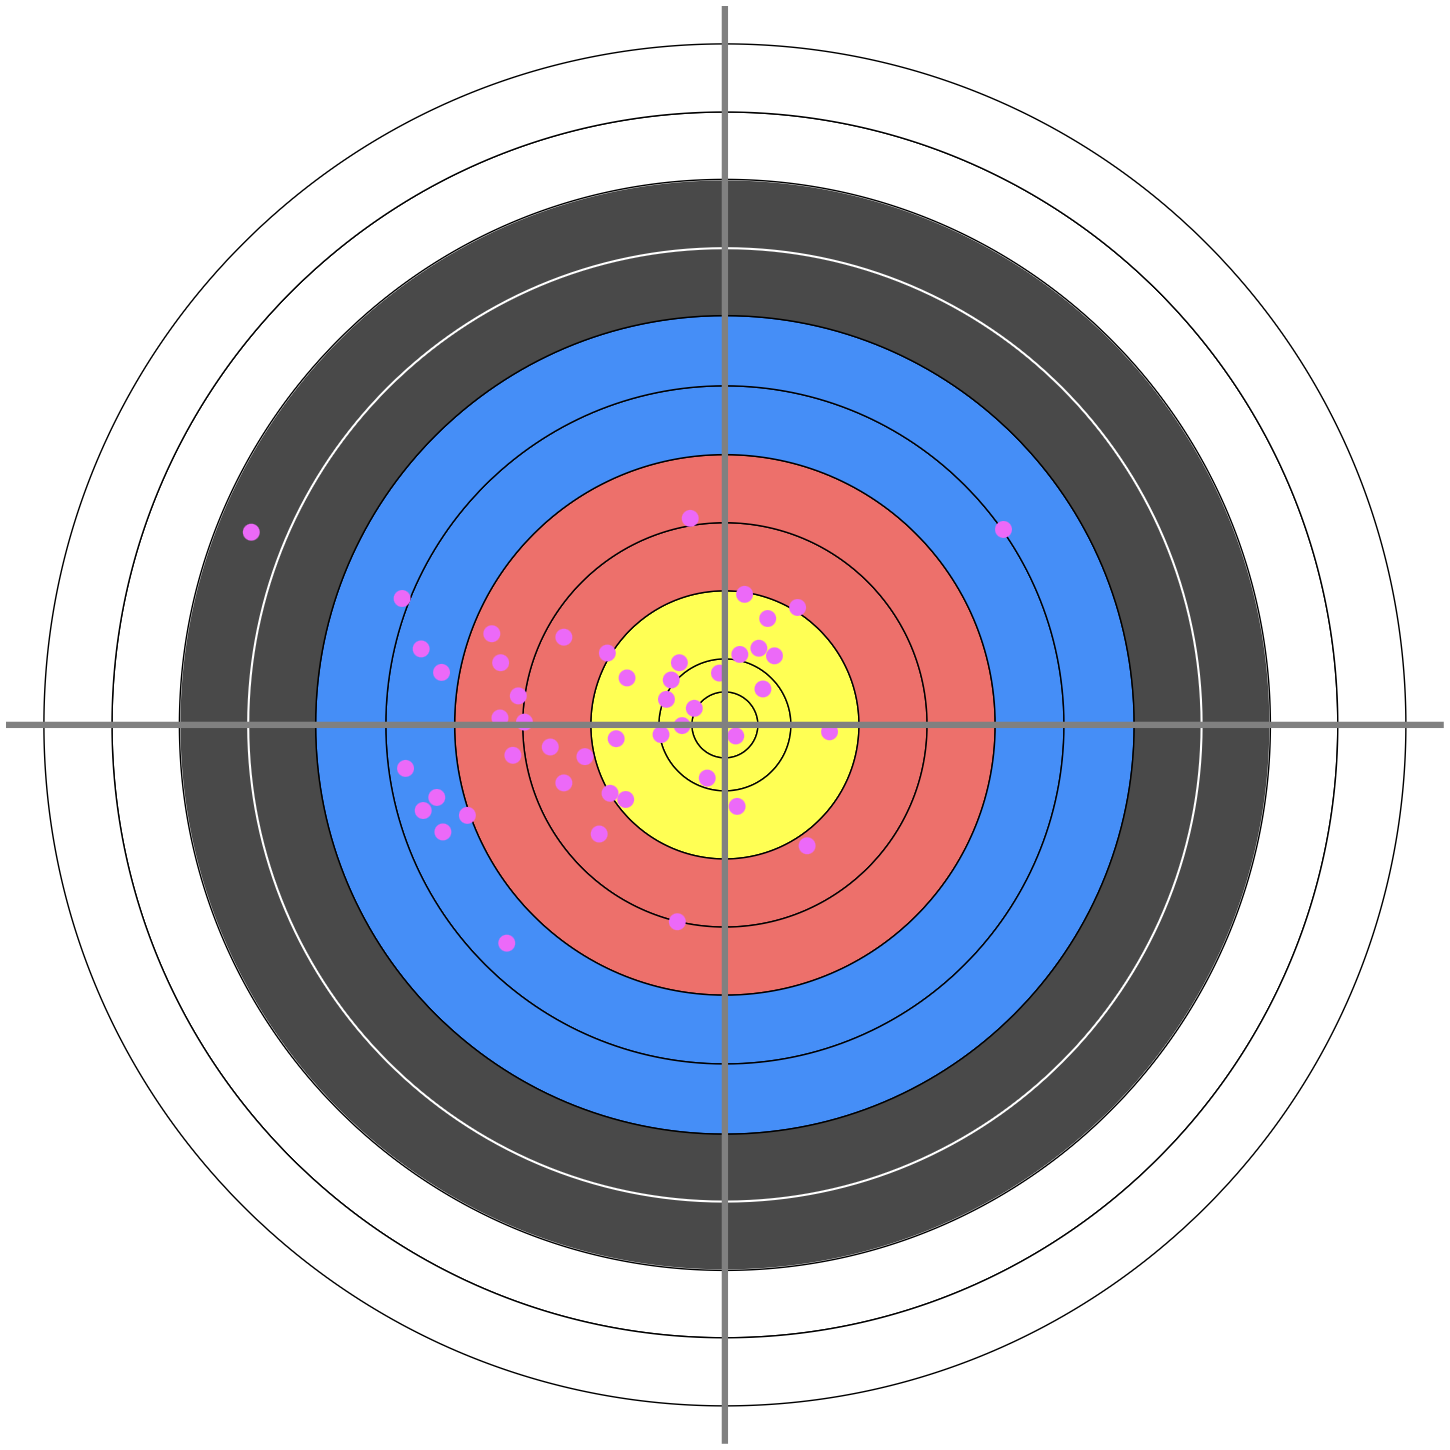
\includegraphics[height=0.825in]{figures/best-date-girl.png}&
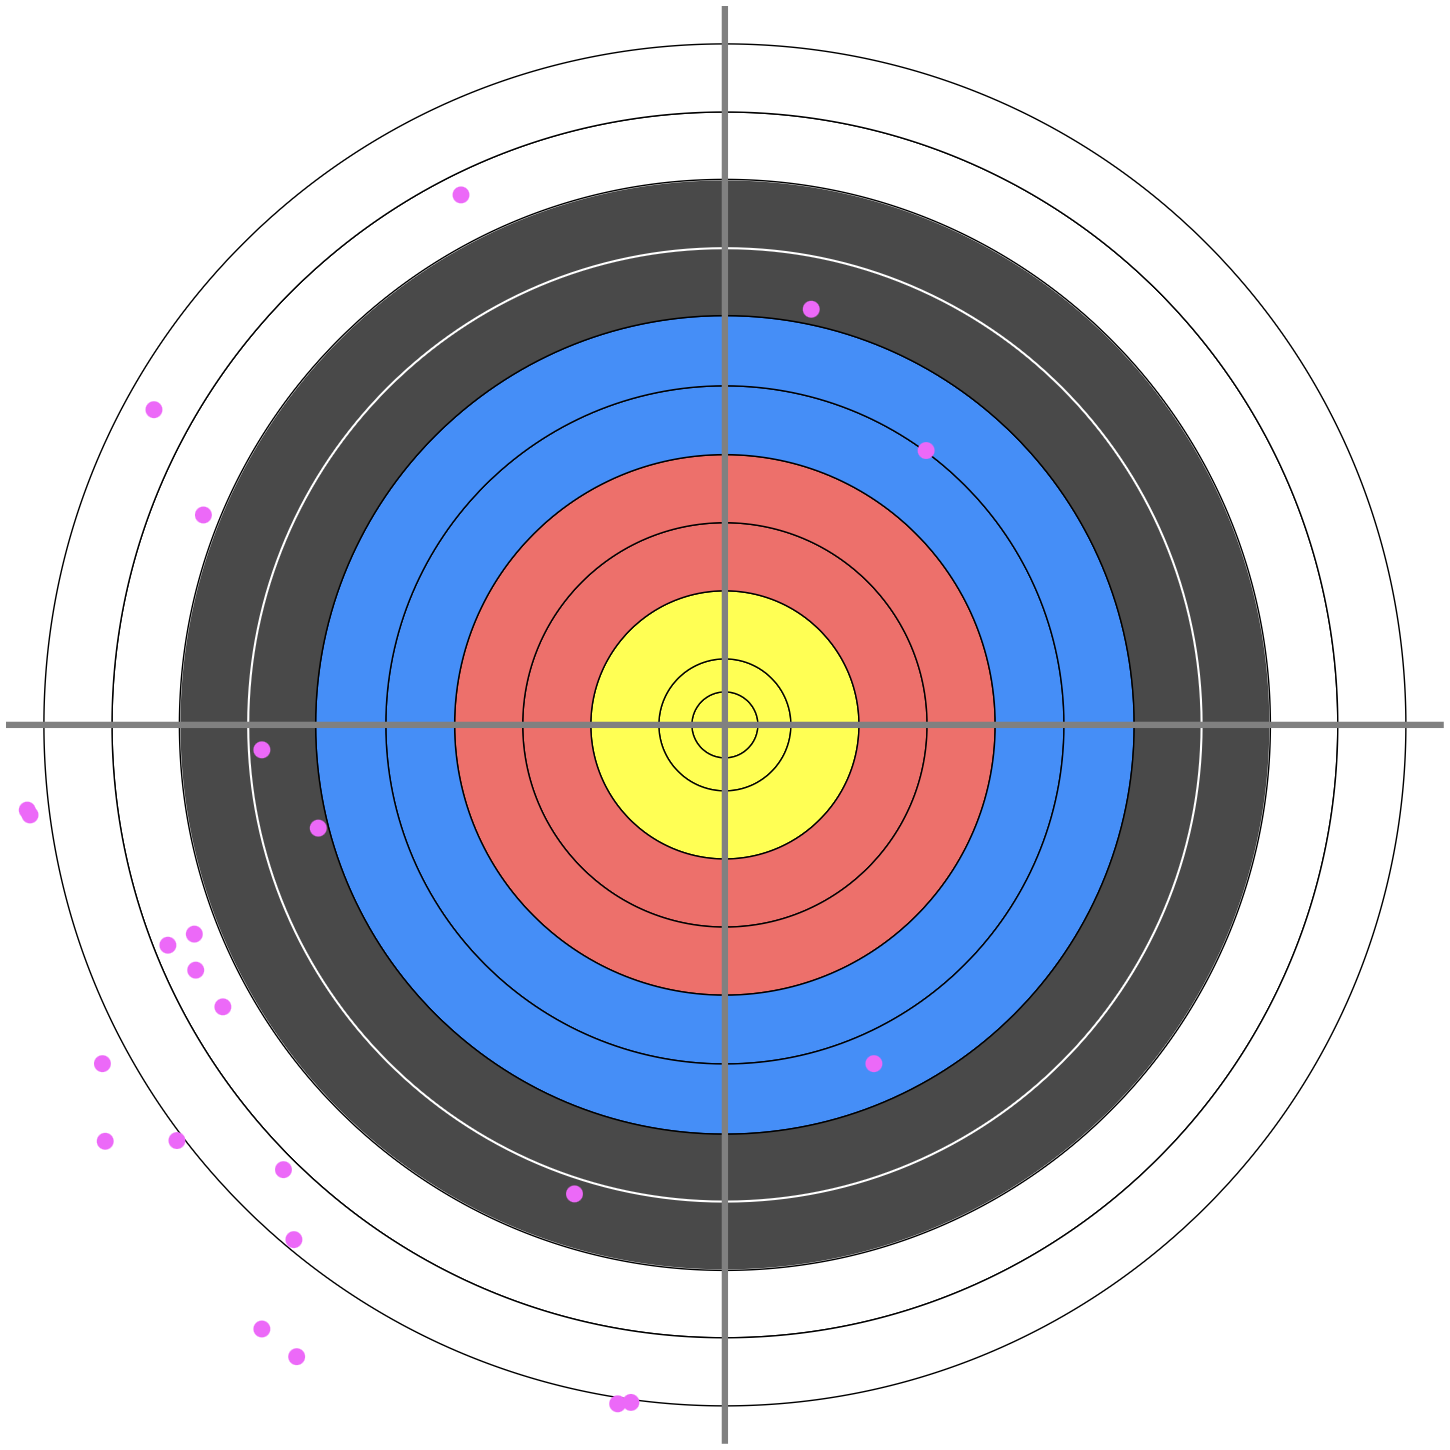
\includegraphics[height=0.825in]{figures/worst-date-girl.png}\\
\mbox{(a)} & \mbox{(b)} & \mbox{} & \mbox{(c)} & \mbox{(d)}
\end{array}$
\end{center}
%\begin{figure*}[htb]
%\begin{center}
%\includegraphics[width=1.0\linewidth]{figures/best-worst-date.pdf}
%\end{center}
\caption{The best and worst dates of the boy (a and b) and the girl (c and d).}
\label{fig:best-worst-date}
\end{figure*}

\section{Results and Discussion}

\subsection{Brushing and Filtering}

The four views of ArcheryVis are dynamically linked to support a comprehensive visualization and comparison of the archery performance data. Two brushing examples are given in Figure~\ref{fig:brushing}. 
In (a) and (b), we brush the temporal view, highlighting the shots in the target view. 
In (c) and (d), we brush the attribute view, and the selected shots that meet query conditions are shown in the target view.
(d) also shows mousing over a shot displaying the tooltip. 

In Figure~\ref{fig:filtering-2}, we show an example of filtering. 
%Both trainees are selected. 
Only the white, blue, and yellow ranges are selected for the point range. 
For the zone, only Zones 1 and 4 are selected. We select a range from November 2022 to January 2023 for the date. The resulting target and temporal views are shown in (c) and (d). 
%
In Figure~\ref{fig:filtering-1}, we show another filtering example. 
Only the black, blue, and red ranges are selected for the point range. 
For the zone, only Zones 2 and 3 are selected. The resulting statistics, target, and attribute views are shown in (b) to (d). 

\subsection{Trainee Comparison}
\label{subsec:tc}

Figure~\ref{fig:overall-target} shows the target views of the two trainees accumulated over the 36 dates. 
Interestingly, the boy shot more arrows in Zones 2 and 4 (the right half of the target), whereas the girl shot more arrows in Zones 1 and 3 (the left half). 
The statistics view reports 678 shots for the boy in Zones 1 and 3 (mean: 5.93) and 1191 in Zones 2 and 4 (mean: 5.64). 
For the girl, there are 1061 shots in Zones 1 and 3 (mean: 5.52) and 769 in Zones 2 and 4 (mean: 5.63). 
This disparity could be explained by how the trainees hold the bow. 
The boy is right-handed, and he holds the bow with his left hand and shoots more at the right half of the target. 
The girl is left-handed and does the opposite. 
Both trainees' performance is slightly better on the half of the target, where fewer arrows are shot. 
If we examine the top/bottom halves of the target, both achieve a better performance on the top half of the target (the means of top and bottom are 5.98 and 5.56 for the boy and 5.82 and 5.33 for the girl). 
Zone-wise, both have the best performance in Zone 1 (294 shots for the boy with a mean of 6.21 and 484 shots for the girl with a mean of 5.89).
%Nevertheless, her performance on the right half of the target is much better than the left half (the means differ by 1.34). 

In Figure~\ref{fig:best-worst-date}, the temporal view shows the best and worst dates for the two trainees, highlighted in (a) to (d). 
The best dates were 5/11/2022 (mean: 8.02) for the boy and 6/1/2022 (mean: 7.90) for the girl. 
The worst dates for both were 7/19/2022 (mean: 2.11 for the boy; mean: 1.67 for the girl). This was the first time they shot 20 yards instead of 10 yards from the target. 
The left ellipse in the temporal view shows that this change has the most significant negative impact on their performance (the mean drops stunningly from 7.92 to 2.11 for the boy and 7.05 to 1.67 for the girl). 
The right ellipse highlights another dip in their performance. 
This was due to their first use of sight, which aids in aligning the bow and arrow with the target. 
It took them a few sessions to adjust. 
As beginners, conditions, such as shooting distance and sight usage, highly influence their performance.  
Finally, with the Pearson linear coefficient of 0.6478, the performances of these two trainees have a moderately positive correlation. 
Their overall means across all dates are similar: 5.74 for the boy and 5.57 for the girl. 

\begin{figure*}[htb]
\begin{center}
$\begin{array}{c@{\hspace{0.025in}}c@{\hspace{0.025in}}c@{\hspace{0.025in}}c}
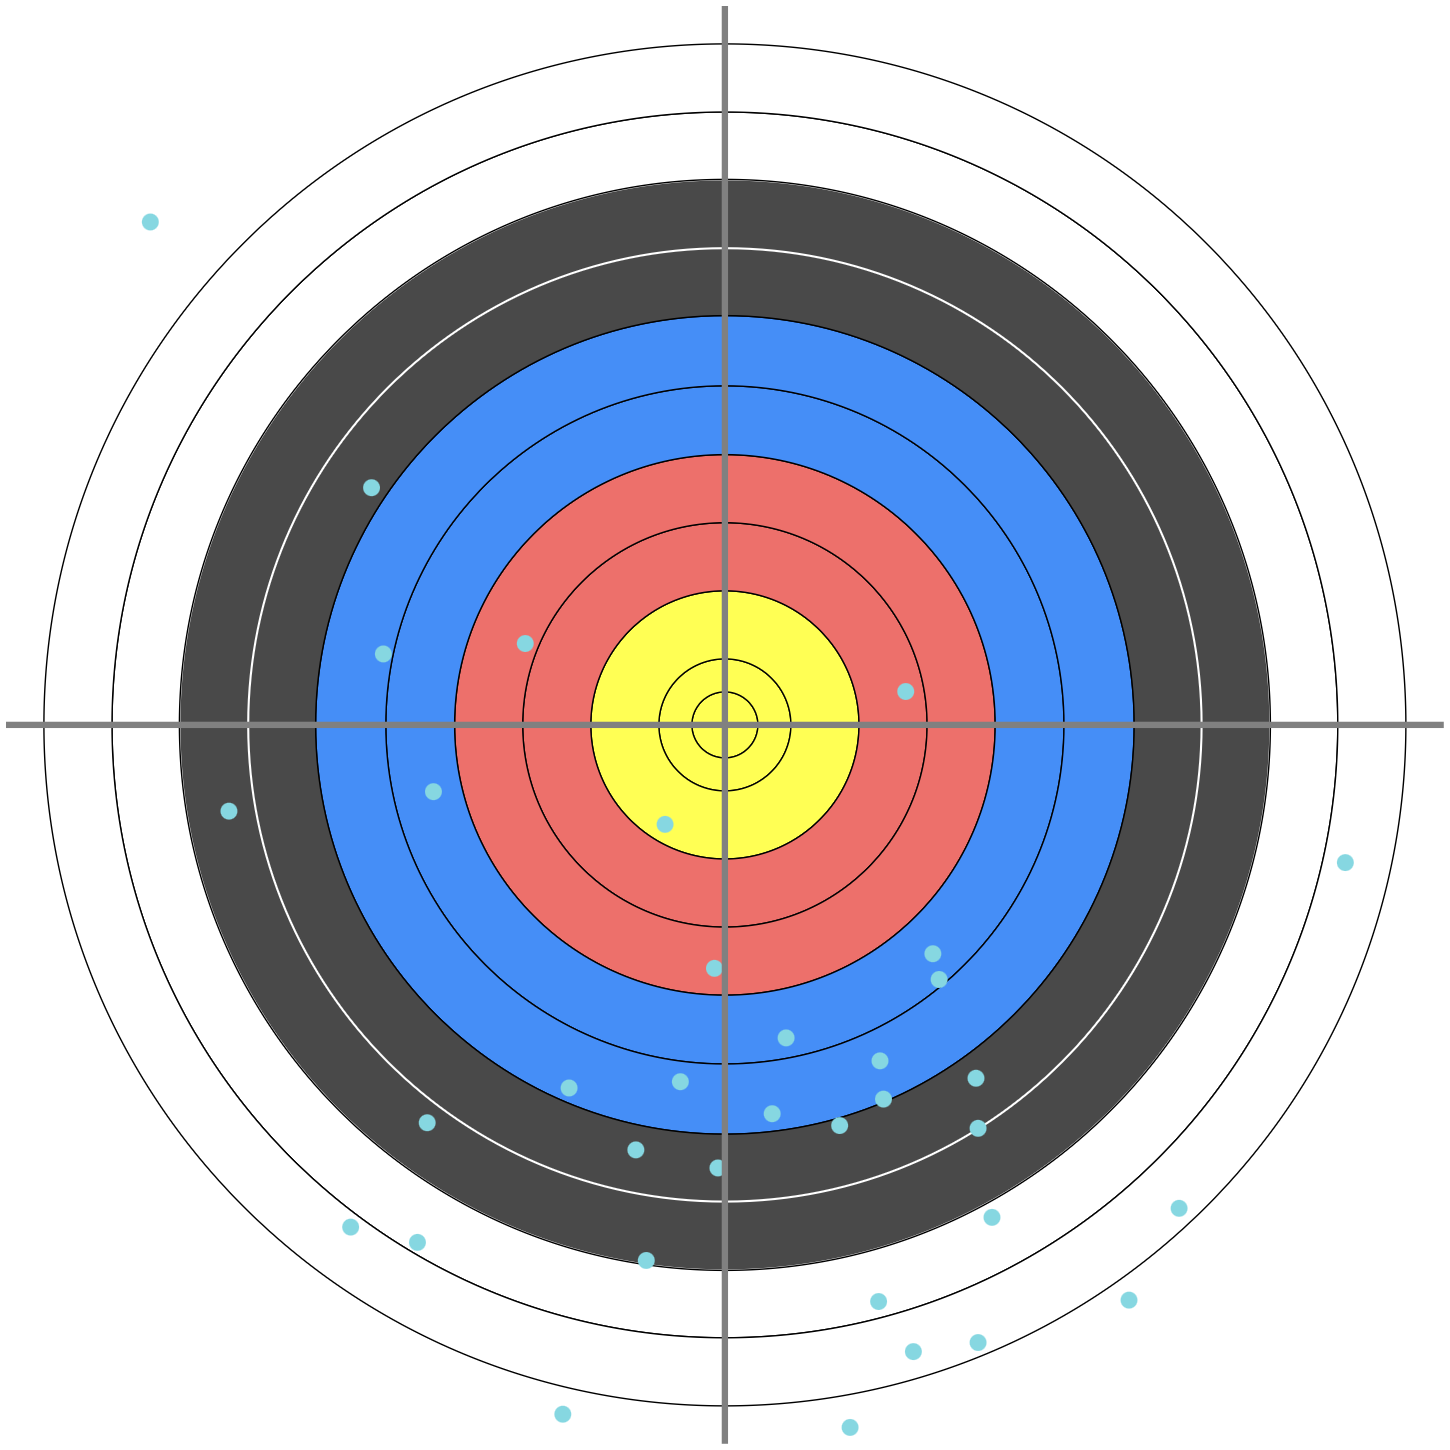
\includegraphics[width=0.235\linewidth]{figures/dispersion-boy-2023-02-11.png}&
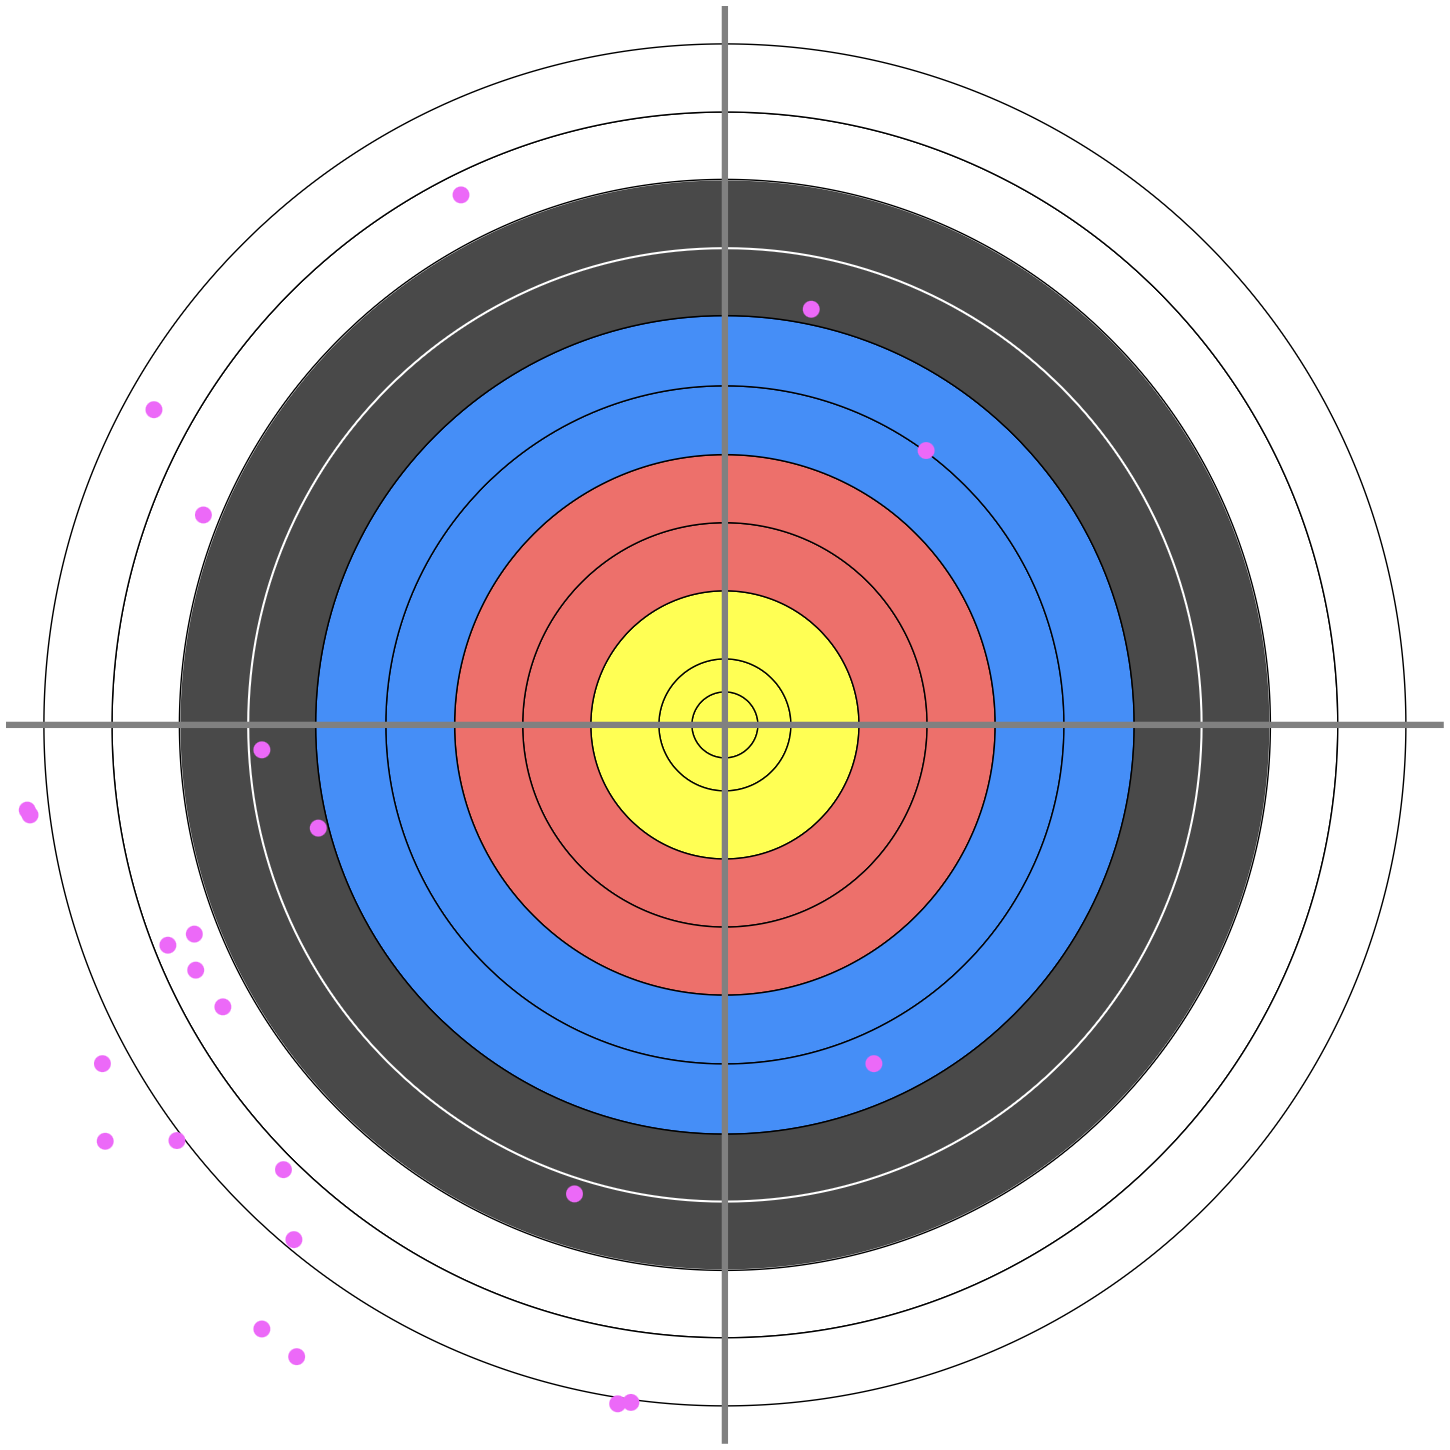
\includegraphics[width=0.235\linewidth]{figures/worst-date-girl.png}&
%\includegraphics[width=0.235\linewidth]{figures/dispersion-girl-2022-07-05.png}&
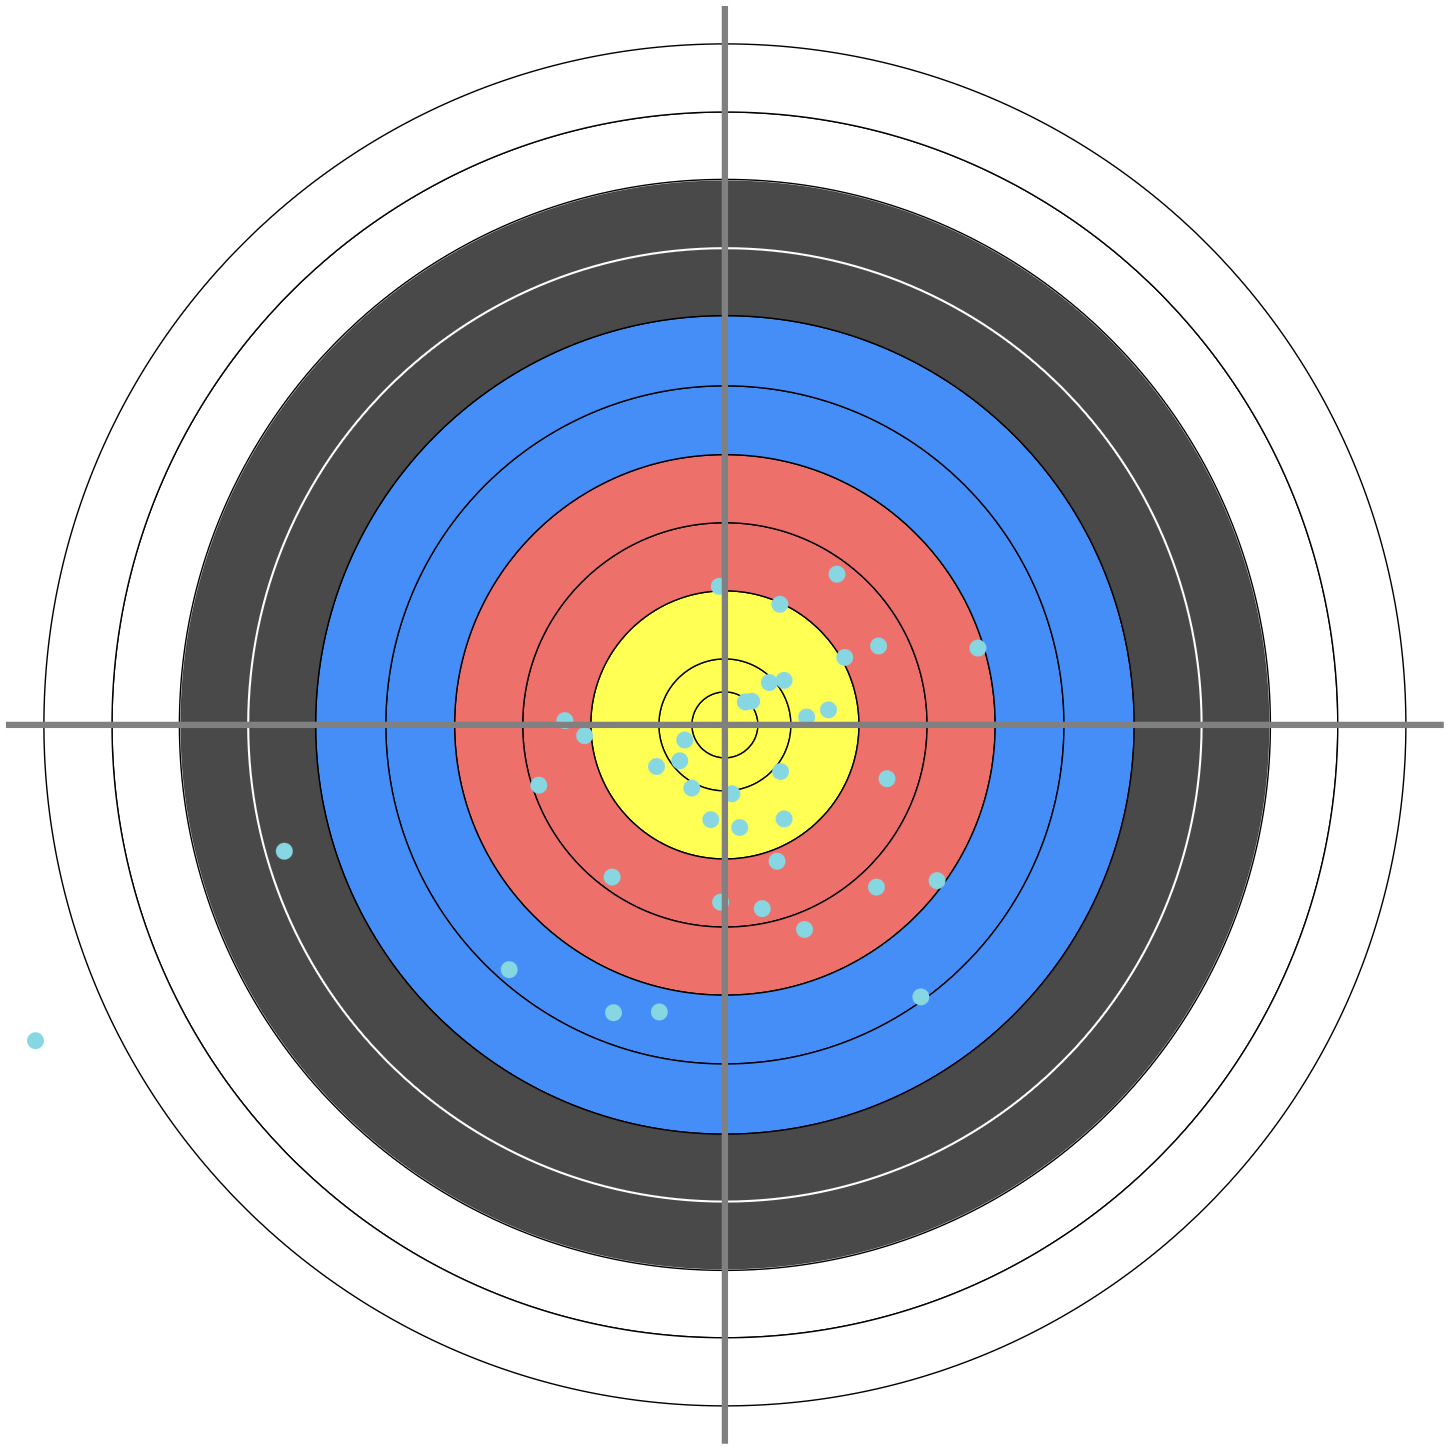
\includegraphics[width=0.235\linewidth]{figures/dispersion-boy-2022-07-05.png}&
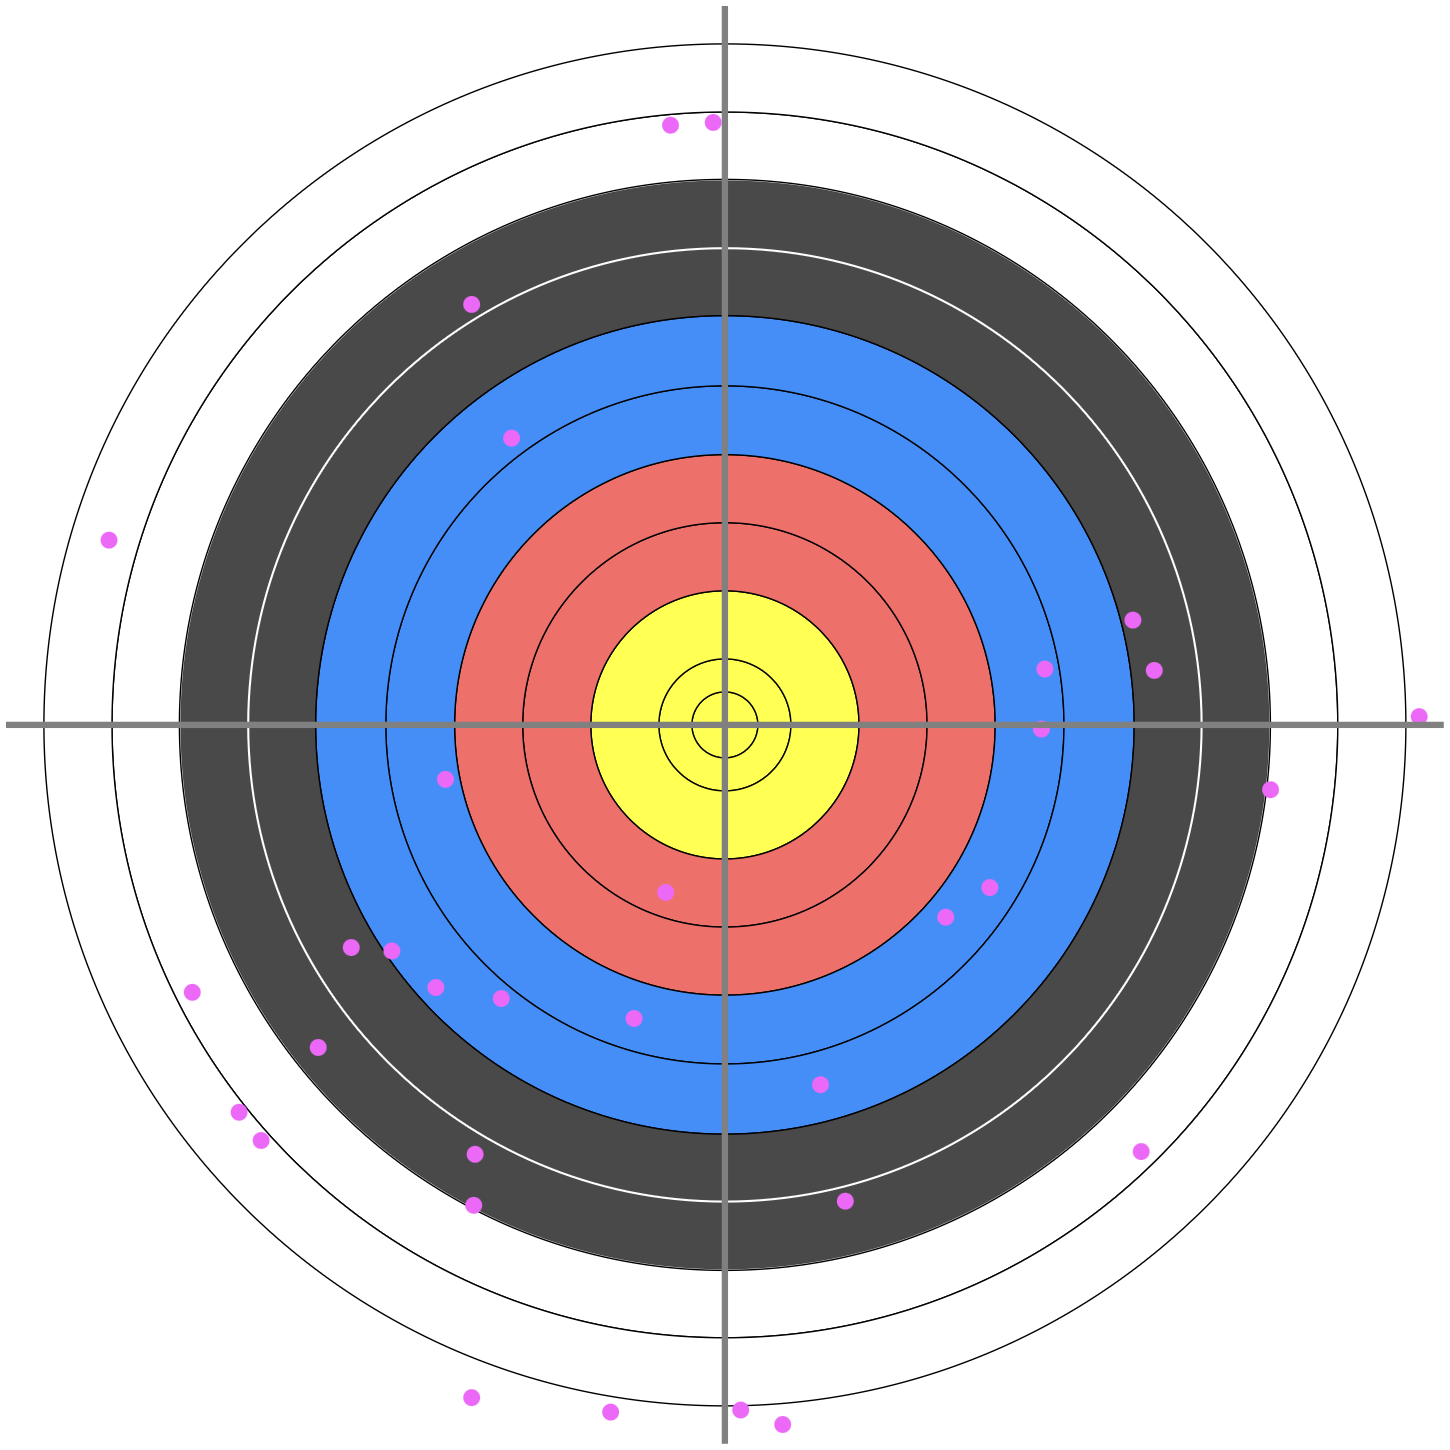
\includegraphics[width=0.235\linewidth]{figures/dispersion-girl-2022-12-13.png}\\
\mbox{(a)} & \mbox{(b)} & \mbox{(c)} & \mbox{(d)}
\end{array}$
\end{center}
\caption{Standard deviation and horizontal and vertical dispersions are unreliable performance indicators.}
\label{fig:dispersion}
\end{figure*}

\subsection{Statistical Measure as Performance Indicator}

As expected, the mean is a reliable performance indicator, but this is not true for other statistical measures. 
%
A large standard deviation may indicate bad performance. 
For example, Figure~\ref{fig:dispersion} (a) shows the boy's target paper of 2/11/2023. 
With a standard deviation of 2.43, this is the boy's second-worst date (mean: 3.69).
However, a small standard deviation does not necessarily indicate good performance. 
For example, Figure~\ref{fig:dispersion} (b) shows the girl's target paper of 7/19/2022. 
With a standard deviation of 1.71, this is the girl's worst date (mean: 1.67).

Horizontal and vertical dispersions are the spreads of the shots along the $x$ and $y$-axes, respectively. 
A large/small difference between them does not imply bad/good performance, as these measures are highly susceptible to outliers. 
Figure~\ref{fig:dispersion} (c) shows the boy's target paper on 7/5/2022. The horizontal and vertical dispersions are, respectively, 1342 and 665 (the difference is 677). This, however, is the boy's second-best date (mean: 7.92). 
In contrast, Figure~\ref{fig:dispersion} (b) shows the girl's target paper on 12/13/2022. The horizontal and vertical dispersions are 1866 and 1855 (the difference is 11). This, however, is the girl's second-worst date (mean: 3.30).

\subsection{Empirical Evaluation}

We initially evaluated ArcheryVis with the two trainees and their trainer. 
We walked through the visual interface and interaction as a group, introducing the available functions. 
Then, they started their free exploration, each taking 10$\sim$15 minutes.
Overall, all of them were satisfied with the functions provided by ArcheryVis. 
In particular, the tool helped them identify some previously unknown findings (e.g., the preference of left/right side of the target in association with right/left-handedness), which we reported in Section~\ref{subsec:tc}. 
They viewed this version of ArcheryVis as a promising start and would like to use it in practice. 

\subsection{Limitations}
%{\bf Limitations}

ArcheryVis focuses on automatic shot detection and scoring as well as the analytical aspects of the tool via visual interface and interaction. 
It does not study varied contributing factors related to archery performance, as discussed in Section~\ref{sec:rw}. 
Also, it does not record the shooting order on the same target paper, which precludes the in-depth chronological performance study within the same training session. 
Furthermore, we do not investigate how the paper size and shooting distance 
%(e.g., the distance for shooting 17"$\times$17" target papers was 10 yards, and that for 25"$\times$25" papers was 20 yards) 
affect the performance. 
Even though the data collected are rather limited, ArcheryVis does offer new capabilities not available in current archery scoring apps. 

\section{Conclusions and Future Work}

We have presented ArcheryVis, a tool for analyzing and visualizing archery performance data. 
Our primary contributions lie in automating shot detection and enabling visual exploration and comparative study of archery trainees. 
Experimental results demonstrate that ArcheryVis achieves its intended goals. 

In the future, we would like to pursue the following directions. 
First, we will further evaluate ArcheryVis with the trainer and trainees to identify potential improvements.  
Second, we will collect more information, including the shooting order and distance, to better help the trainer and trainees analyze archery performance data. 
Third, we will refine our process to support the continued use of the developed tool. The local archery shop/club could provide such a service so that trainees can conveniently review their data, and the trainer can access the digital data of all the trainees for scalable visual analysis.  
We need to address the scalability issue with many trainees and a sizable training data record. 
Finally, besides the current web-based visual interface, we will develop an app version of the tool for wide dissemination.

\subsubsection{Acknowledgements} 
This research was supported in part by the U.S.\ National Science Foundation through grants DUE-1833129, IIS-1955395, IIS-2101696, and OAC-2104158. The authors thank Tram Trinh and Janet Meng, who contributed to the project's development, and the anonymous reviewers for their comments.
%
% ---- Bibliography ----
%
% BibTeX users should specify bibliography style 'splncs04'.
% References will then be sorted and formatted in the correct style.
%
\bibliographystyle{splncs04}
\bibliography{template}

\end{document}
